\documentclass[12pt]{article}
\usepackage[utf8]{inputenc}
\usepackage{amsmath}
\usepackage{amsfonts}
\usepackage{amssymb}
\usepackage{graphicx}
\usepackage{booktabs}
\usepackage{geometry}
\geometry{margin=1in}
\usepackage{float}
\usepackage{array}     % For p{width} column type (paragraph columns)
\usepackage{subcaption}

\usepackage{threeparttable} % Highly recommended for professional table notes
\usepackage{xcolor}

\usepackage{amsmath}   % for \underset, aligned math
\usepackage{amssymb}   % for \mathbb{1} and \mathbb{R}
\usepackage{bbm}       % alternatively, for \mathbbm{1} (bolder indicator)
\DeclareMathOperator*{\argmin}{arg\,min}


\newcommand{\E}{\mathbb{E}}
\newcommand{\I}{\mathcal{I}}
\usepackage{setspace}
\onehalfspacing

\bibliographystyle{apacite}
\usepackage[nosectionbib,numberedbib]{apacite}

\usepackage{natbib}
%\bibliographystyle{abbrvnat}
\setcitestyle{authoryear,open={(},close={)}}
\usepackage{breakcites}

\usepackage[affil-it]{authblk}

\usepackage{xcolor}
\usepackage{hyperref}
\hypersetup{
    colorlinks  = true,
    citecolor   = darkgray,      % color for citations
    linkcolor   = blue,      % color for internal links
    urlcolor    = blue       % color for URLs
}

\title{Measuring Macroeconomic and Financial Uncertainty: Impact for the Mexican Economic Growth Expectation}
\author{Jes\'us L\'opez-P\'erez\thanks{e-mail: \texttt{jesus.lopezperez32@gc.cuny.edu}, Department of Economics, The Graduate Center\\ The City University of New York}}



\date{May 30, 2026}

\begin{document}

\maketitle


\section{Introduction}
Central banks when making monetary policy must account for various risks including real economic factors and financial risks. When doing a balance of risks they weigh both downside risks --production, unemployment-- and upside risks --inflation. In addition, financial risk are usually associated with high volatility, that can be seen as an endogenous response to the business cycle or as an exogenous impulse to it \citep{ludvigson2021uncertainty}. 

Measuring uncertainty arises as a problem relevant for decision makers. Three main visions to uncertainty stand out in the literature: the Economic Policy Uuncertainty \cite{baker2016measuring}, which tries to answer how uncertain is the policy environment that households and firms face; the VIX index used in finance addresses the question of how much financial markets expect asset prices to fluctuate; while, another view is the one from \cite{jurado2015measuring} (JLN - hencefort) which is concerned about how unpredictable is the macroeconomy, and \cite{ludvigson2021uncertainty} (LMN - henceforth) about what are the roles of macroeconomic and financial uncertainty.

The problem for the forecaster is then extended from the usual GDP growth point estimate to the broader task of estimating lower, middle and higher quantiles. These additional estimates can be later used for assessing the conditional mean of GDP growth on increased volatility of economic and financial conditions. The question at hand is thus:\textit{ what is the worst economic growth outcome what we should expect with given probability?.} This has been tackled in the relevant study by \cite{adrian2019vulnerable}. They develop a framework --Growth-at-Risk (GaR)-- that allow to obtain the empirical quantile distribution based on preliminary lower, middle and upper quantiles. 

In this research I focus on the estimation of the empirical quantile distribution of IGAE growth ---proxy for monthly GDP--- conditional on uncertainty measures for the Mexican economy. The question is relevant because, unlike the US FOMC, the Mexican central bank does not have the dual mandate of keeping low inflation and achieving potential GDP growth. Banco de Mexico (Banxico) has the only mandate of keeping inflation low; thus, its assessment of risks is not the same as in the US economy.

IGAE is a monthly indicator built with most of the data used to compute quarterly GDP and has become relevant in the analysis of short-term economic situation \citep{elizondo2019estimaciones}. In Section \ref{sec:univariate}, I present this variable and conduct unit-root tests, test for endogenous structural breaks, and decompose the series into cycle $+$ permanent components. 


To construct the indices described before, in Section \ref{sec:multivariate} I build on the data of \cite{corona2022timely}. In particular, I rely on the panel that considers the most relevant information for the Mexican economy, which has two key characteristics: contains only public information, which allows reproducibility of results; it contains information that is timely available, as it is designed to generate nowcasts in the first 15 calendar days after the month closes. In Section~\ref{sec:DFM} I employ the same methodology of \cite{corona2022timely} to estimate a Dynamic Factors Model (DFM). This methodology is the one currently used by the Mexican national statistics agency, INEGI, to produce timely estimates on a regular basis\footnote{\url{https://www.inegi.org.mx/investigacion/ioae/}}. 


With DFM in hand, in Section~\ref{sec:MU-FU} I proceed to employ the JLN methodology to estimate uncertainty indices, which are later employed for the remaining of the paper. As a natural continuation of the JLN methodology, in Section~\ref{sec:SVAR} I proceed to estimate a SVAR to test the ordering of uncertainty to real economic activity and viceversa, followed by an analysis for their relevance into forecasting and impulse-response function. As a robustness check, in Section~\ref{sec:LP} IRF are estimated using local projections following \cite{jorda2005estimation}. 

The Section~\ref{sec:GaR} then estimates the yearly growth rate of IGAE conditional on the uncertainty indices constructed in previous sections and the current economic conditions. Finally, the Section~\ref{sec:coint} presents an analysis of real economic activity and labor markets, along with the uncertainty indices measured before. 

The paper conclusions and directions for future research are presented in Section~\ref{sec:conclusions}.

\section{Summary of Methodologies}
\subsection*{Dynamic Factors Model}
Let $\mathbf{x}_t = (x_{1t}, \ldots, x_{Nt})'$ be an $N \times 1$ vector of
stationary macroeconomic and financial series observed at $t = 1, \ldots, T$.
The DFM decomposes each variable into a common and an idiosyncratic component:

\begin{equation}\label{eq:dfm}
  x_{it} = \boldsymbol{\lambda}_i' \mathbf{F}_t + e_{it}, \qquad
  i = 1,\ldots,N,
\end{equation}

\noindent where $\mathbf{F}_t = (F_{1t},\ldots,F_{rt})'$ is an $r \times 1$
vector of latent common factors, $\boldsymbol{\lambda}_i$ is the corresponding
vector of factor loadings, and $e_{it}$ is the idiosyncratic disturbance,
assumed to be weakly correlated across $i$ and uncorrelated with
$\mathbf{F}_t$. The number of factors $r$ is selected using the
\cite{bai2002determining} information criteria:

\begin{equation}\label{eq:bai-ng}
  \mathrm{IC}_p(k) = \ln V(k, \hat{\mathbf{F}}^k) + k \cdot g(N,T),
\end{equation}

\noindent where $V(k,\hat{\mathbf{F}}^k)$ is the average residual variance
under $k$ factors and $g(N,T)$ is a penalty function that increases with the
panel dimensions. Factors and loadings are estimated by the two-step principal-components method of \cite{doz2012quasi}.


\subsection*{Measuring uncertainty}
Following \cite{jurado2015measuring}, uncertainty for series $j$ at horizon $h$ is defined as the conditional
volatility of its unforeseeable component. We obtain

$e_{it} = x_{it} - \mathbf{F}_t'\boldsymbol{\lambda}_i$
$e_{it}$.


\begin{equation}\label{eq:jln}
  \mathcal{U}^y_{jt}(h) =
    \sqrt{\mathbb{E}\!\left[
      \bigl(y_{j,t+h} - \hat{\mathbb{E}}[y_{j,t+h} \mid \mathcal{I}_t]
      \bigr)^2 \,\Big|\, \mathcal{I}_t
    \right]},
\end{equation}

\noindent where $\hat{\mathbb{E}}[y_{j,t+h} \mid \mathcal{I}_t]$ is the
best linear forecast of $y_{j,t+h}$ using information
$\mathcal{I}_t = \{\mathbf{F}_s, \mathbf{x}_s\}_{s \leq t}$. 


Then, estimate a GARCH(1,1) model. For each variable $i$, fit: $e_{it} = \sigma_{it}\,\eta_{it}, \qquad \eta_{it} \sim \mathit{iid}(0,1)$
\[
\sigma^2_{it} = \omega_i + \alpha_i\,e^2_{i,t-1} + \beta_i\,\sigma^2_{i,t-1}
\]
with $\omega_i > 0$,\ $\alpha_i, \beta_i \geq 0$,\ $\alpha_i + \beta_i < 1$.

where 
$\sigma_{it}$ is the conditional standard deviation of the unforeseeable component, what JLN call the measure of uncertainty.

Next, aggregate each of the volatility estimates into MU and FU

$MU_t = \frac{1}{N_{{M}}}\sum_{i \in {M}} \sigma_{it}, \quad$
$FU_t = \frac{1}{N_{{F}}}\sum_{i \in {F}} \sigma_{it}$

Both indexes are standardized to zero mean and unit variance.

\subsection*{Structural VAR}

Let $\mathbf{X}_t = (MU_t,\; IGAE_t,\; FU_t)'$. The reduced-form VAR($p$) is:

\begin{equation}\label{eq:var}
  \mathbf{X}_t = \mathbf{c} + \sum_{j=1}^{p} \mathbf{A}_j \mathbf{X}_{t-j}
                + \mathbf{B}\mathbf{d}_t + \mathbf{u}_t,
  \qquad \mathbf{u}_t \sim (0, \boldsymbol{\Sigma}_u),
\end{equation}

\noindent where $\mathbf{d}_t$ is a vector of impulse dummies absorbing the
structural breaks at 2009/05 and 2020/04, and $p = 4$ is selected by
likelihood ratio tests. Structural shocks $\boldsymbol{\varepsilon}_t$ are
recovered via Cholesky decomposition
$\boldsymbol{\Sigma}_u = \mathbf{P}\mathbf{P}'$, so that
$\boldsymbol{\varepsilon}_t = \mathbf{P}^{-1}\mathbf{u}_t$ with
$\mathbb{E}[\boldsymbol{\varepsilon}_t \boldsymbol{\varepsilon}_t'] =
\mathbf{I}_3$. The recursive ordering (Ordering A) restricts $MU_t$ from
responding to contemporaneous $IGAE_t$ or $FU_t$ shocks; Ordering B
($FU$ first) is used as a robustness check.


\subsection*{Growth-at-Risk}
The quantile estimation, following \cite{adrian2019vulnerable} the conditional distribution of IGAE growth is characterized through quantile regressions at horizons $h \in \{1,3,6,12\}$ months. While the impulse responses and local projections obtained in the Structural VAR allow to identify the mean effect of uncertainty shocks on IGAE growth, the quantile regression allows to assess whether uncertainty 
disproportionately compresses the lower tail of the growth distribution, this under-stress scenario is the most relevant for risk assessment.

For each quantile level $\tau \in (0,1)$ and forecast horizon 
$h \in \{1, 3, 6, 12\}$ months, we estimate:

\begin{equation}\label{eq:gar}
  Q_\tau\!\left( IGAE_{t+h} \mid \mathbf{z}_t \right)
  = \alpha_{\tau,h}
  + \beta^{MU}_{\tau,h}\, MU_t
  + \beta^{FU}_{\tau,h}\, FU_t
  + \gamma_{\tau,h}\, IGAE_t,
\end{equation}

\noindent where $g_{t+h}^{(h)}$ denotes the year-on-year growth rate of 
IGAE at horizon $h$, $g_t$ is the contemporaneous growth rate (a 
persistence control), and $\mathbf{z}_t = (MU_t, FU_t, g_t)'$. The 
quantile regression coefficients are obtained by minimising the 
asymmetric loss function

\begin{equation}
    \hat{\beta}_{\tau} = \underset{\beta_{\tau} \in \mathbbm{R}^{k}}{\argmin}
    \sum_{t=1}^{T-h} \left(
    \tau \cdot \mathbbm{1}_{(y_{t+h} \geq x_t \beta)}
    \left| y_{t+h} - x_t \beta_{\tau} \right|
    +
    (1 - \tau) \cdot \mathbbm{1}_{(y_{t+h} < x_t \beta)}
    \left| y_{t+h} - x_t \beta_{\tau} \right|
    \right)
\end{equation}



\textcolor{black}{Following \cite{adrian2019vulnerable}, the direct $h$-period ahead local projections are estimated via quantile regressions.} I estimate the conditional distribution of IGAE growth via quantile regressions at horizons $h \in \left\lbrace 1, 3, 6, 12 \right\rbrace $ months. I report the 5th percentile of the conditional distribution as the Growth-at-Risk summary statistic. \footnote{The parametric skewed-$t$ step of Adrian et al. (2019) is omitted as the quantiles of interest are estimated directly."}



\section{Data}
\subsection{Univariate analysis: IGAE}\label{sec:univariate}

Figure \ref{fig:igae_panels} shows the evolution of Mexican Global Economic Activity Indicator (IGAE acronym from Spanish) for the period January 2004 to December 2024. \cite{inegi_gdp_quarterly_2026}.  The top panel shows the evolution of the variable in levels, where the index is constructed to compare real economic activity in 2018 pesos. 
The middle panel shows the month-over-month variation, this transformation allows to capture short-term movements and remove the trend of the variable. The bottom panel shows the year-over-year changes, this reflects medium term variation and allows to remove seasonality effects.


\begin{figure}[htbp]
  \centering
  \begin{subfigure}{0.7\textwidth}
    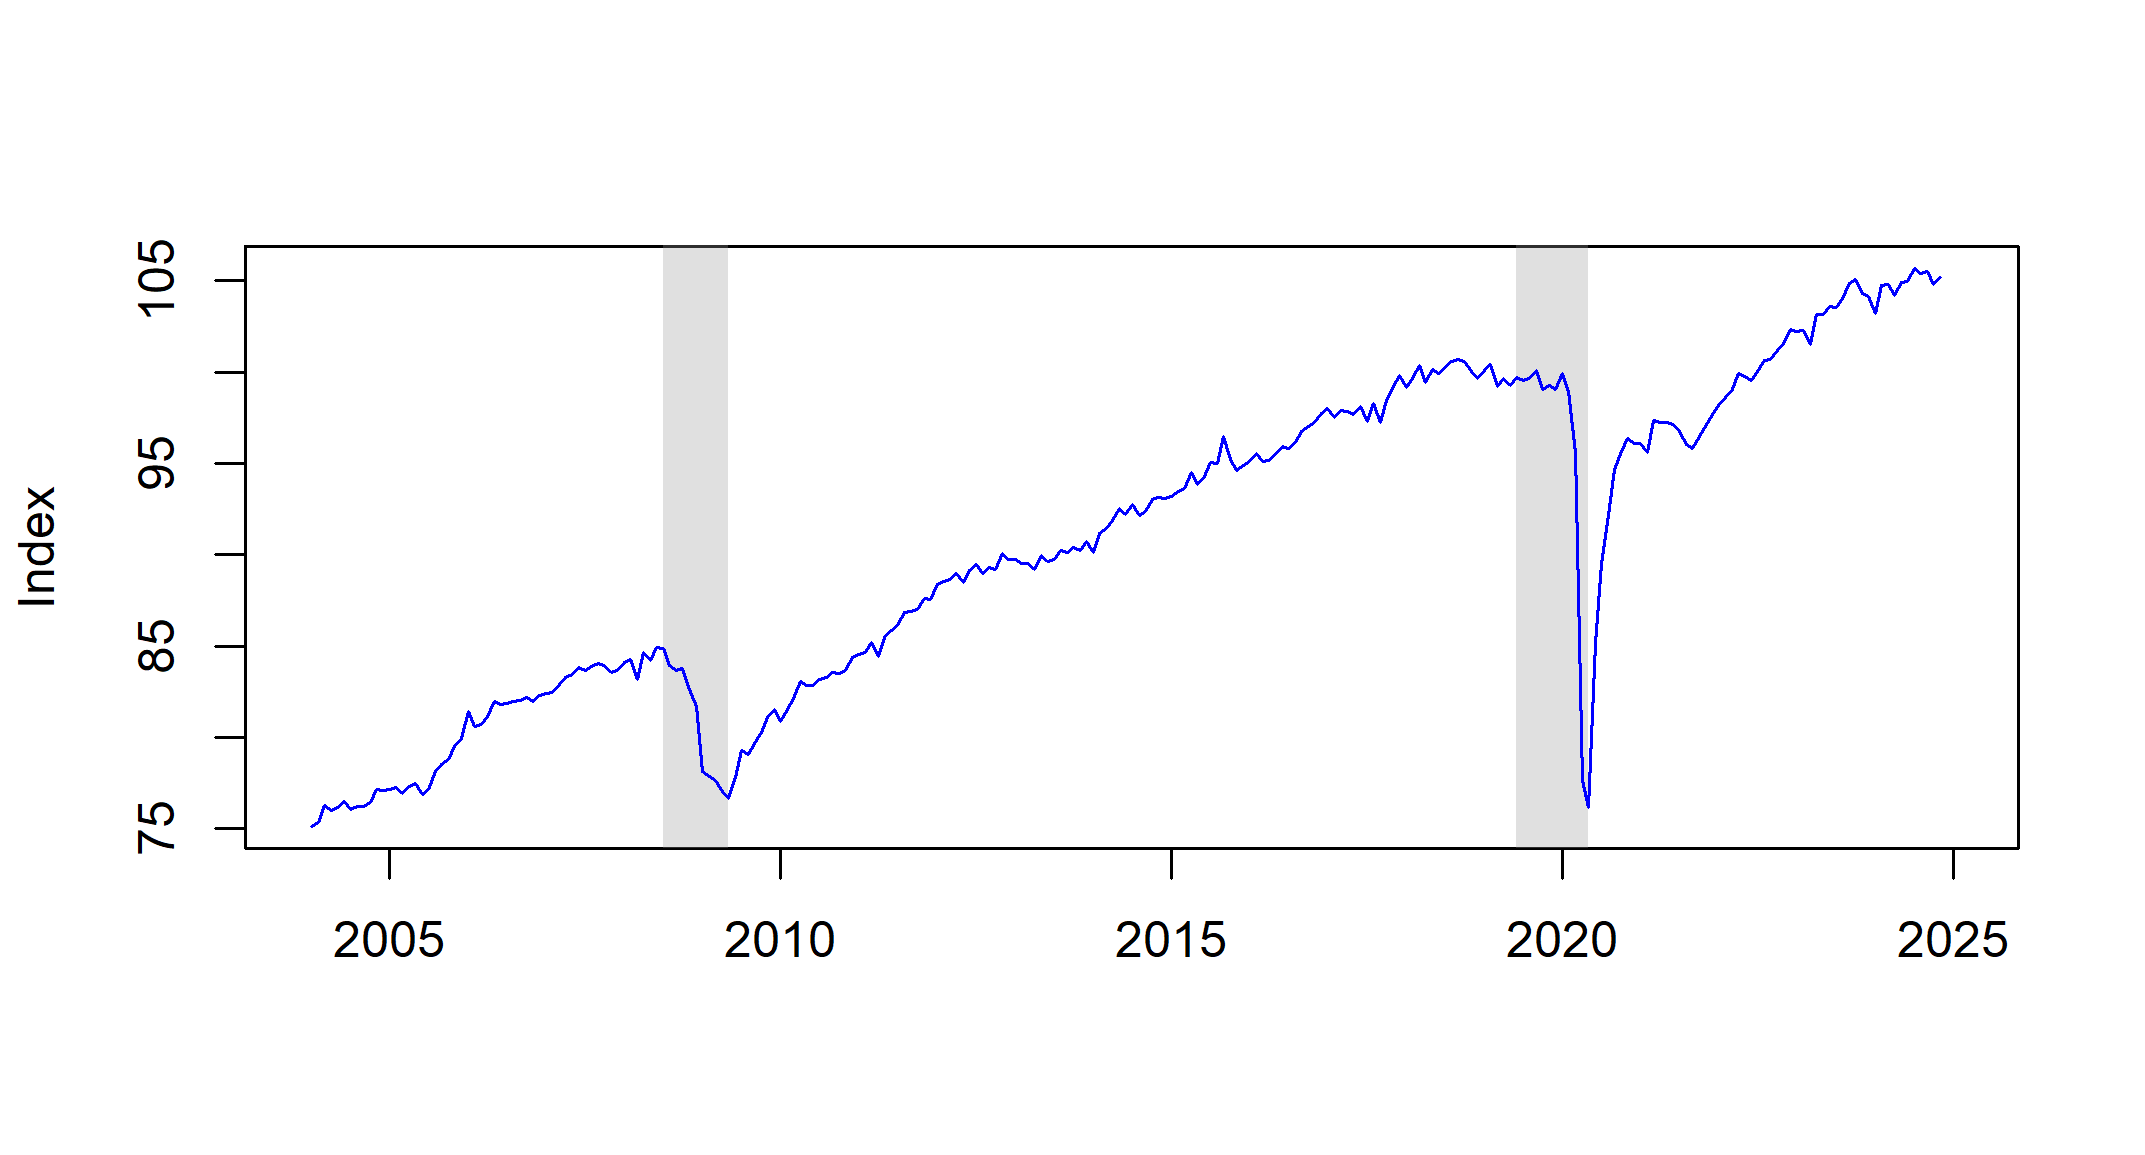
\includegraphics[width=\textwidth]{../ioae_assesment/outputs/eda/igae_lev.png}
    \caption{IGAE index (2018 = 100)}
    \label{fig:igae_levels}
  \end{subfigure}


  \begin{subfigure}{0.7\textwidth}
    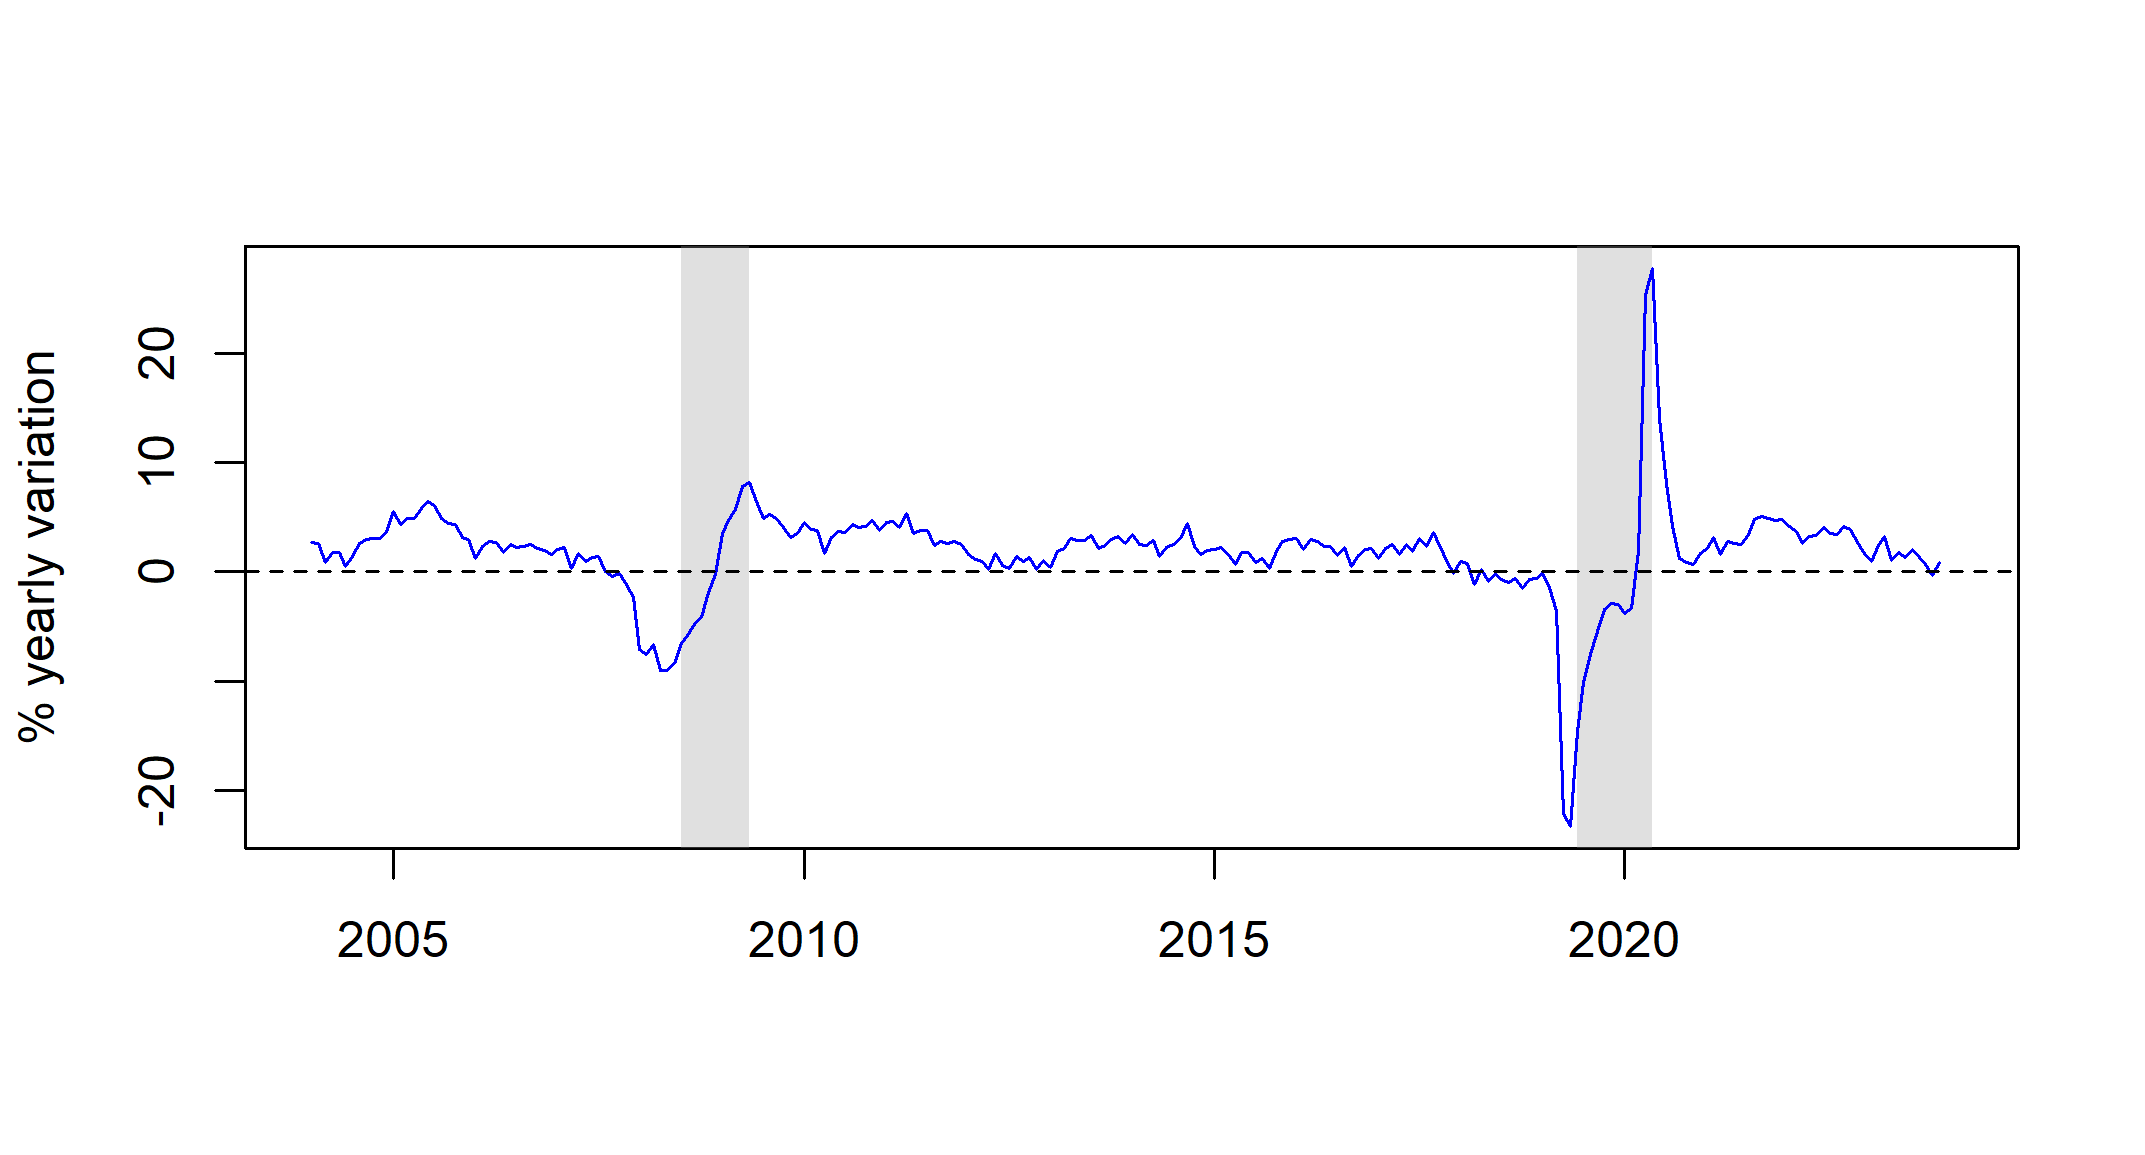
\includegraphics[width=\textwidth]{../ioae_assesment/outputs/eda/igae_mv.png}
    \caption{Month-on-month growth (\%)}
    \label{fig:igae_yoy}
  \end{subfigure}

  \begin{subfigure}{0.7\textwidth}
    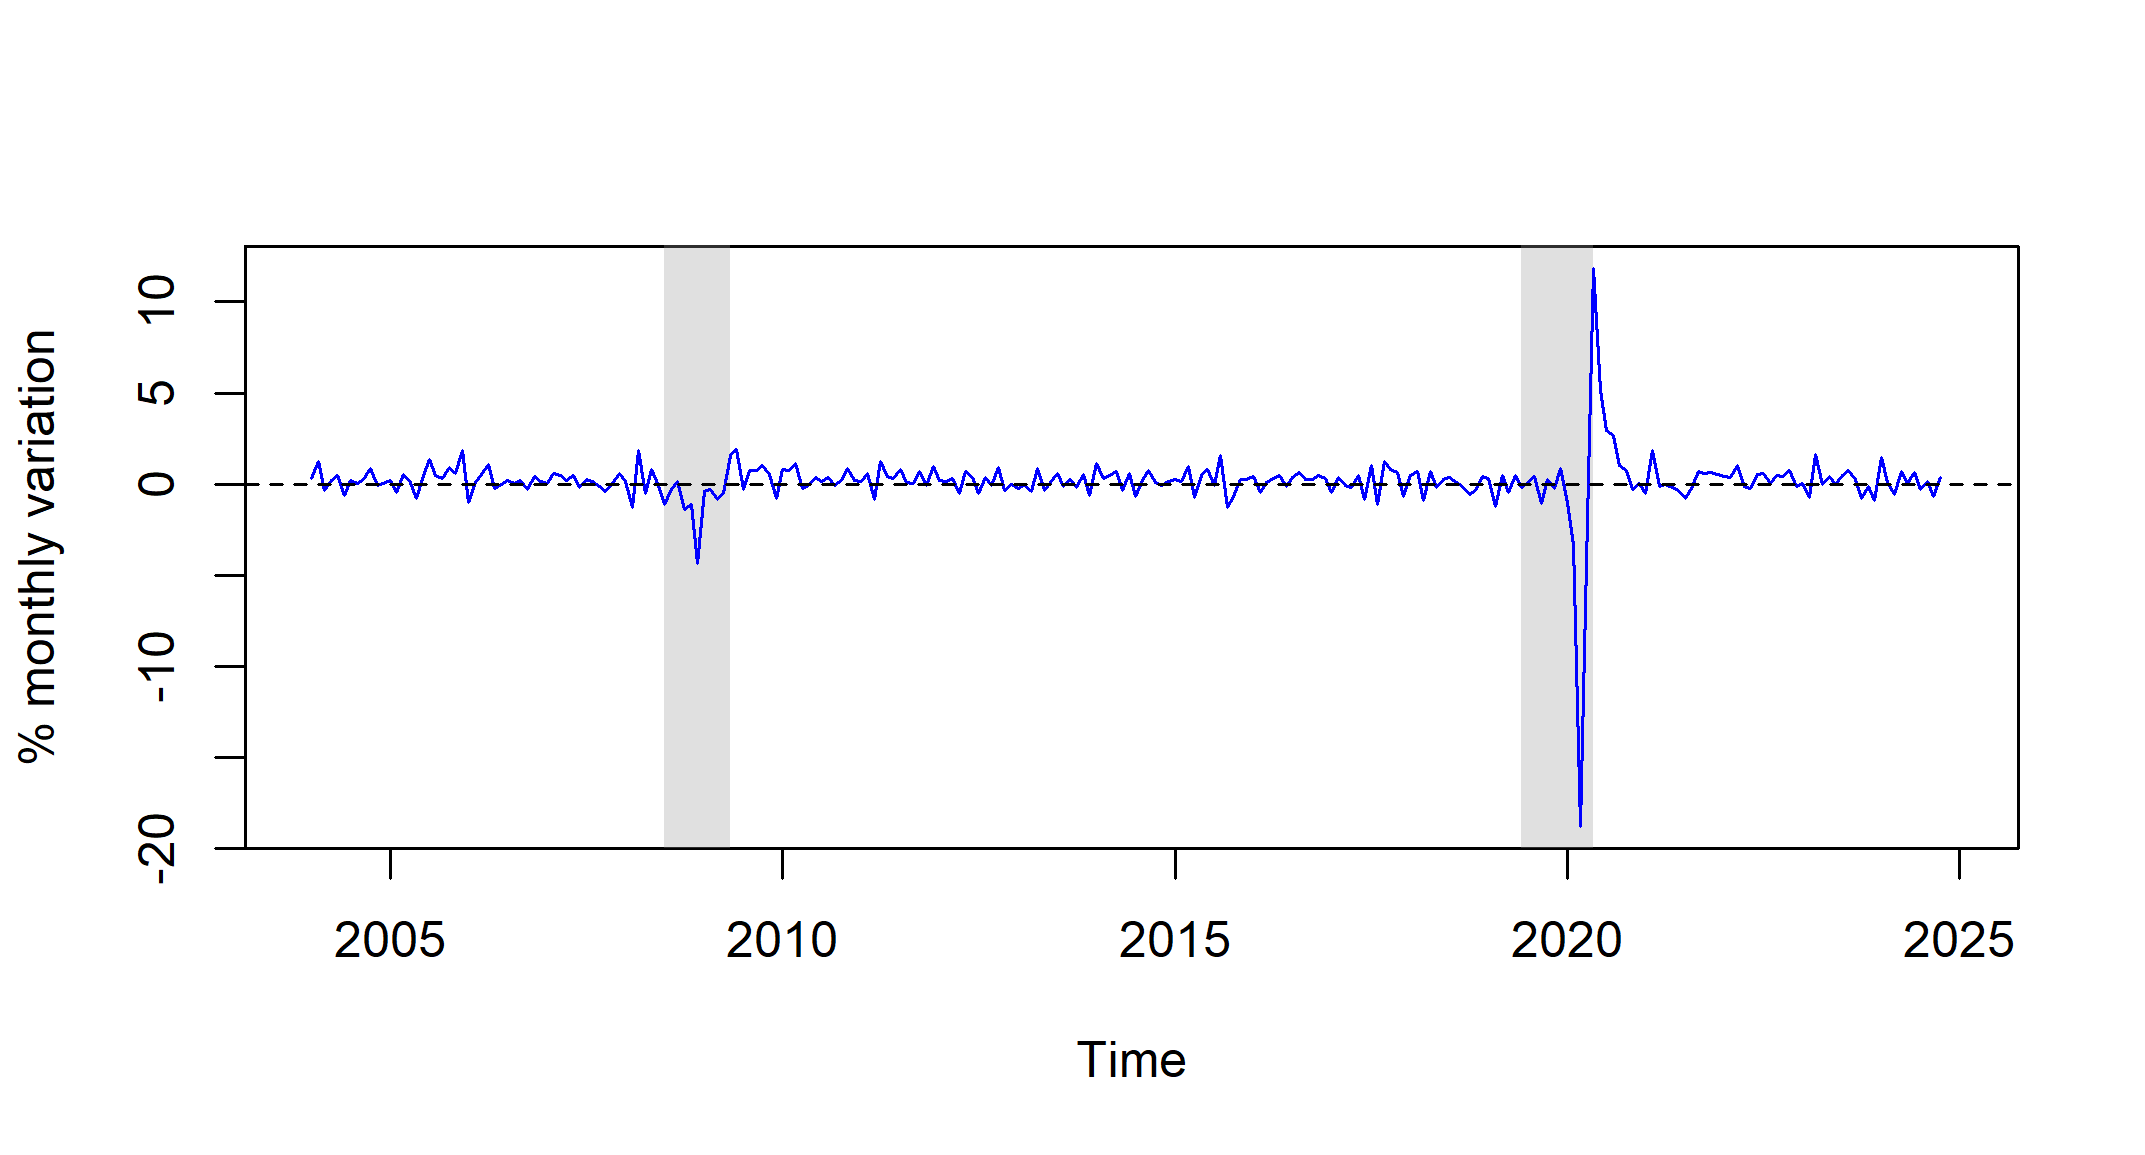
\includegraphics[width=\textwidth]{../ioae_assesment/outputs/eda/igae_yoy.png}
    \caption{Year-on-year growth  (\%)}
    \label{fig:igae_mv}
  \end{subfigure}

  \caption{INEGI's General Economic Activity Index (IGAE in Spanish), Mexico, 2004--2025.
           Shaded areas indicate IMEF-dated recession periods (GFC: Jul 2008--May 2009; COVID: Jun 2019--May 2020).}
  \label{fig:igae_panels}
\end{figure}


To account for the presence of unit root, I conduct three statistical tests Augmented Dickey-Fuller (ADF), Phillips-Perron (PP) and Kwiatkowski-Phillips-Schmidt-Shin (KPSS) tests; the results from these tests are presented in Table \ref{tab:unit-root-tests}. For levels evidence is mixed — ADF/PP reject the unit root at 5\% but KPSS also rejects stationarity at 5\%.  Monthly variation is $I(0)$: ADF and PP reject the unit root, and KPSS does not reject stationarity at any conventional level. Finally, yearly variation is also $I(0)$: ADF and PP reject unit root present, both below the 1\% critical value, and KPSS fails to reject stationarity at any conventional level.

We incorporate the results from unit-root tests in two ways. First, this validates using IGAE monthly growth rate in the VAR analysis, since this series is $I(0)$ and
satisfies the stationarity requirement for VAR stability. Second, we  use IGAE yearly variation in the Growth-at-Risk analysis presented in section \ref{sec:GaR}, since it is
also $I(0)$ but also allows to smooth over transitory monthly noise and makes a better target for forecasting purposes at different horizons.


\begin{table}
\centering
\caption{IGAE: Unit-root tests}\label{tab:unit-root-tests}
\begin{tabular}{llrrrr}
\hline
\textbf{Series} & \textbf{Test} & \textbf{Stat} & \textbf{CV 1\%} & \textbf{CV 5\%} & \textbf{CV 10\%} \\
\hline
\multicolumn{6}{l}{\textit{ADF — H$_0$: unit root; reject if stat $<$ CV}} \\
\hline
Levels           & ADF &  $-4.792$ & $-3.980$ & $-3.420$ & $-3.130$ \\
Monthly var.     & ADF & $-13.030$ & $-3.460$ & $-2.880$ & $-2.570$ \\
Yearly var.       & ADF &  $-6.179$ & $-3.460$ & $-2.880$ & $-2.570$ \\
\hline
\multicolumn{6}{l}{\textit{PP — H$_0$: unit root; reject if stat $<$ CV}} \\
\hline
Levels           & PP  &  $-3.761$ & $-3.998$ & $-3.429$ & $-3.138$ \\
Monthly var.     & PP  & $-11.934$ & $-3.458$ & $-2.873$ & $-2.573$ \\
Yearly var.       & PP  &  $-4.785$ & $-3.459$ & $-2.874$ & $-2.573$ \\
\hline
\multicolumn{6}{l}{\textit{KPSS — H$_0$: stationary; reject if stat $>$ CV}} \\
\hline
Levels           & KPSS &  $0.203$ &  $0.216$ &  $0.176$ &  $0.146$ \\
Monthly var.     & KPSS &  $0.022$ &  $0.739$ &  $0.574$ &  $0.463$ \\
Yearly var.       & KPSS &  $0.080$ &  $0.739$ &  $0.574$ &  $0.463$ \\
\hline
    \multicolumn{6}{l}{
    \parbox{0.65\textwidth}{\footnotesize \textit{Notes:} ADF - Augmented-Dickey Fuller test, PP - Phillip-Perron test, KPSS - Kwiatkowski-Phillips-Schmidt-Shin test. ADF and PP include trend for levels, drift only for growth rates. }} \\
\end{tabular}
\end{table}


\subsubsection*{Structural breaks}\label{sec:structural-breaks}

To account for the presence of both exogenous and endogenous structural breaks I conduct the appropriate statistical tests. 

First, I take care of the dates about the recessions marked by the IMEF's Mexican Business Cycle Dating Committee \citep{comite2025}. I apply Chow test at the known recession turning points --- this test whether the regression coefficients shift at a \textit{pre-specified }date under the null of parameter stability, the results are presented in Table \ref{tab:exog}. Structural breaks are present in the \textit{level} of IGAE but not in its monthly growth rate.

Three conclusions arise from this analysis. First, the 2009 and 2020 recessions produced permanent level shifts in economic activity. Second, monthly variation does not reflect this shifts is structurally stable across both episodes ($p > 0.10$). Third, first-differencing simultaneously removes the unit root and the structural breaks.


\begin{table}[H]
\centering
\begin{threeparttable}
\caption{Exogenous Structural Breaks}\label{tab:exog}
\begin{tabular}{llrr}
\hline
\textbf{Series} & \textbf{Date} & \textbf{F} & \textbf{p-val} \\
\hline
\multicolumn{4}{l}{\textit{IGAE levels}} \\
\hline
Levels & 2009/05 & \textcolor{black}{243.86} & \textcolor{black}{0.000} \\
Levels & 2020/05 & \textcolor{black}{115.32} & \textcolor{black}{0.000} \\
\hline
\multicolumn{4}{l}{\textit{IGAE monthly variation}} \\
\hline
Monthly var. & 2009/05 & 0.271 & 0.603 \\
Monthly var. & 2020/05 & 1.657 & 0.199 \\
\hline
\end{tabular}
\begin{tablenotes}
    \small
    \item \textit{Notes:} Chow parameter stability tests;  null hypothesis ($H_0$) no structural break at the specified candidate date. Candidate breakdown dates identified by the IMEF business cycle recession chronology. %Levels regressions include a constant and a linear time trend; monthly variations evaluate the first-difference of the log-transformed series.
\end{tablenotes}
\end{threeparttable}
\end{table}


Next, I take care of the presence of endogenous breaks. For which I use Bai-Perron and Zivot-Andrews tests. The Bai-Perron methodology searches for multiple unknown breakpoints
jointly, selecting the number of breaks by BIC and estimating their dates simultaneously, while the Zivot-Andrews test extends the standard ADF by allowing for
a single endogenous break in either the intercept, trend, or both. 
 Results are as follows. First, Table~\ref{tab:Bai-Perron} shows that Bai-Perron identifies six level shifts in IGAE, concentrated around macro events: 2006/01 (Post-NAFTA adjustment), 2011/05 (Euro-area sovereign crisis), 2014/03 ( Oil price decline), 2016/08 (US electoral uncertainty), 2020/02 COVID-19 recession, 2022/03 Post-pandemic inflation surge. Monthly growth rate shows no structural breaks ---the BIC selects $m = 0$. Next, Table \ref{tab:Zivot-Andrews} allows to see that Zivot-Andrews confirms break at 2020/04 ($-5.70 < -5.57$) and rejects the unit root for monthly variation ($-12.80 < -5.34$). 

Considering both the results from exogenous and endogenous tests, I added impulse-type dummies in the VAR estimation only at 2009/05 and 2020/04 without distorting the own series dynamics. 

\begin{table}[H]
\centering
\begin{threeparttable}
\caption{Bai-Perron (BIC-optimal partition)}\label{tab:Bai-Perron}
\begin{tabular}{lcc}
\hline
 & \textbf{Levels} & \textbf{Monthly var.} \\
\hline
Optimal breaks ($m$) & 6 & 0 \\
BIC & 1234 & 963.7 \\
\hline
\end{tabular}
\begin{tablenotes}
    \small
    \item \textit{Notes:} Endogenous structural break test results following the Bai-Perron (2003) methodology for IGAE. %The "Optimal breaks ($m$)" represents the number of partitions that minimize the Bayesian Information Criterion (BIC), allowing for up to a maximum of five breaks with a 15\% trimming percentage.  "Levels" specification includes a constant and a deterministic time trend; "Monthly variation" refers to the first-difference of the series. A result of $m=0$ indicates that the BIC-optimal model is a single linear process without structural shifts.
\end{tablenotes}

\end{threeparttable}
\end{table}


\begin{table}[H]
\centering
\begin{threeparttable}
\caption{Zivot-Andrews }\label{tab:Zivot-Andrews}
\begin{tabular}{lrrl}
\hline
\textbf{Series} & \textbf{Stat} & \textbf{CV 1\%} & \textbf{Break} \\
\hline
Levels       & $-5.697$ & $-5.57$ & 2020/02 \\
Monthly var. & $-12.797$ & $-5.34$ & 2020/04 \\
\hline
\end{tabular}
\begin{tablenotes}
    \small
    \item \textit{Notes:} Zivot-Andrews (1992) unit root test, to endogenously determine the single most significant structural break date in the series. Both test statistics reject the unit root null hypothesis at the 1\% significance level. %Null hypothesis ($H_0$) states that the series contains a unit root without any structural breaks. The specification allows for a structural break in both the intercept (level) and the trend for "IGAE Levels," and a break in the intercept for "Monthly Variation" (the first-difference of the log-transformed series). Both test statistics reject the unit root null hypothesis at the 1\% significance level, indicating that both series are stationary after accounting for the endogenously identified shift.
\end{tablenotes}
\end{threeparttable}
\end{table}

\subsubsection*{PT decomposition}

To perform BN decomposition, I estimate various ARIMA models to identify the best fit, these models are summarized in Table~\ref{tab:ARIMA-models}. The results show that the AIC gap between ARIMA(2,1,0) and ARIMA(2,1,2) is very small, only 1.2 points. I select upon the BIC criterion for parsimony. The ARIMA model is $\Delta y_t = \mu + \phi_1\Delta y_{t-1} + \phi_2\Delta y_{t-2} + \varepsilon_t$
which has the following BN decomposition closed form:
\begin{equation}\label{eq:bn_cycle}
  C_t^{\mathrm{BN}}
  = \frac{(\phi_1+\phi_2)(\Delta y_t - \mu)
          + \phi_2(\Delta y_{t-1}-\mu)}
         {1 - \phi_1 - \phi_2},
\end{equation}
with the permanent component $\tau_t^{\mathrm{BN}} = y_t - C_t^{\mathrm{BN}}$. Additional comparison is made with the HP filter using $\lambda = 14400$ given that the frequency of data is monthtly. The cyclical components are shown in Figure~\ref{fig:cycle}: the cycle obtained under the HP being more volatile than the one with BN. The permanent components are shown in Figure~\ref{fig:trend}: here HP trend component is clearly smoother than the BN, it even to not captures the large decline in the COVID pandemic. 


\begin{table}[H]
\centering
\begin{threeparttable}
\caption{ARIMA model selection for IGAE decomposition}\label{tab:ARIMA-models}
\begin{tabular}{lllll}
\hline
         Model &  N&   Loglik&       AIC&       BIC\\
\hline
ARIMA(2,1,0)& 250& 679.17& -1352.35& \textbf{-1341.78}\\
ARIMA(1,1,0)& 250& 669.50& -1335.00& -1327.96\\
ARIMA(2,1,2)& 250& 681.78& \textbf{-1353.56}& -1335.95\\
\hline
\end{tabular}
\begin{tablenotes}
    \small
    \item \textit{Notes:} Alternative Autoregressive Integrated Moving Average (ARIMA($p,d,q$)) specifications for IGAE.The ARIMA(2,1,0) model is selected for the historical decomposition to prevent overfitting, as dictated by the stricter penalty function of the BIC.
% The parameters $p$, $d$, and $q$ denote the autoregressive order, the degree of first-differencing required for stationarity ($d=1$), and the moving average order, respectively. AIC and BIC denote the Akaike Information Criterion and the Bayesian Information Criterion, respectively. Bold values indicate the optimal specification minimizing the respective information criterion. 
\end{tablenotes}
\end{threeparttable}
\end{table}



\begin{figure}[H]
\centering
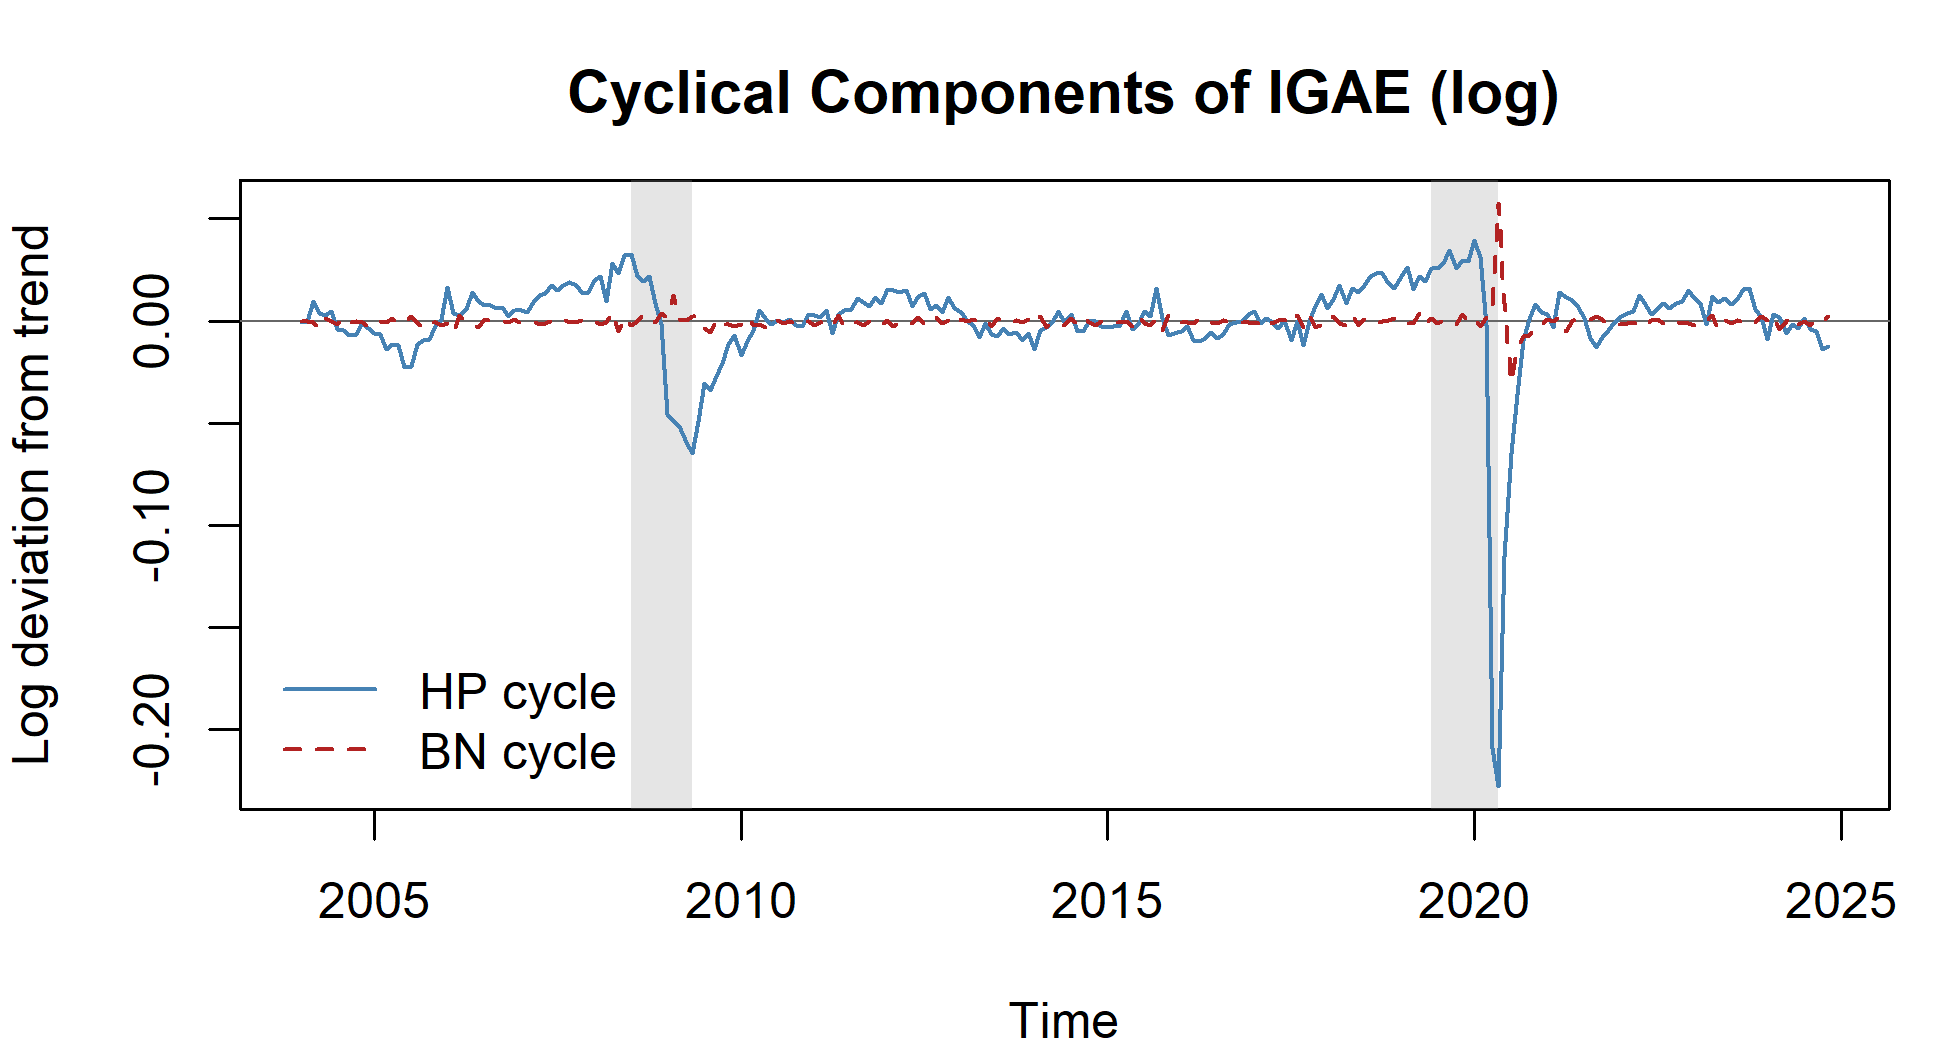
\includegraphics[width=\textwidth]{../ioae_assesment/outputs/eda/igae_cycle.png}
\caption{IGAE estimated cyclical components. HP filter using $\lambda= 1600$, BN using ARIMA(2,1,0) specification.}\label{fig:cycle}
\end{figure}

\begin{figure}[H]
\centering
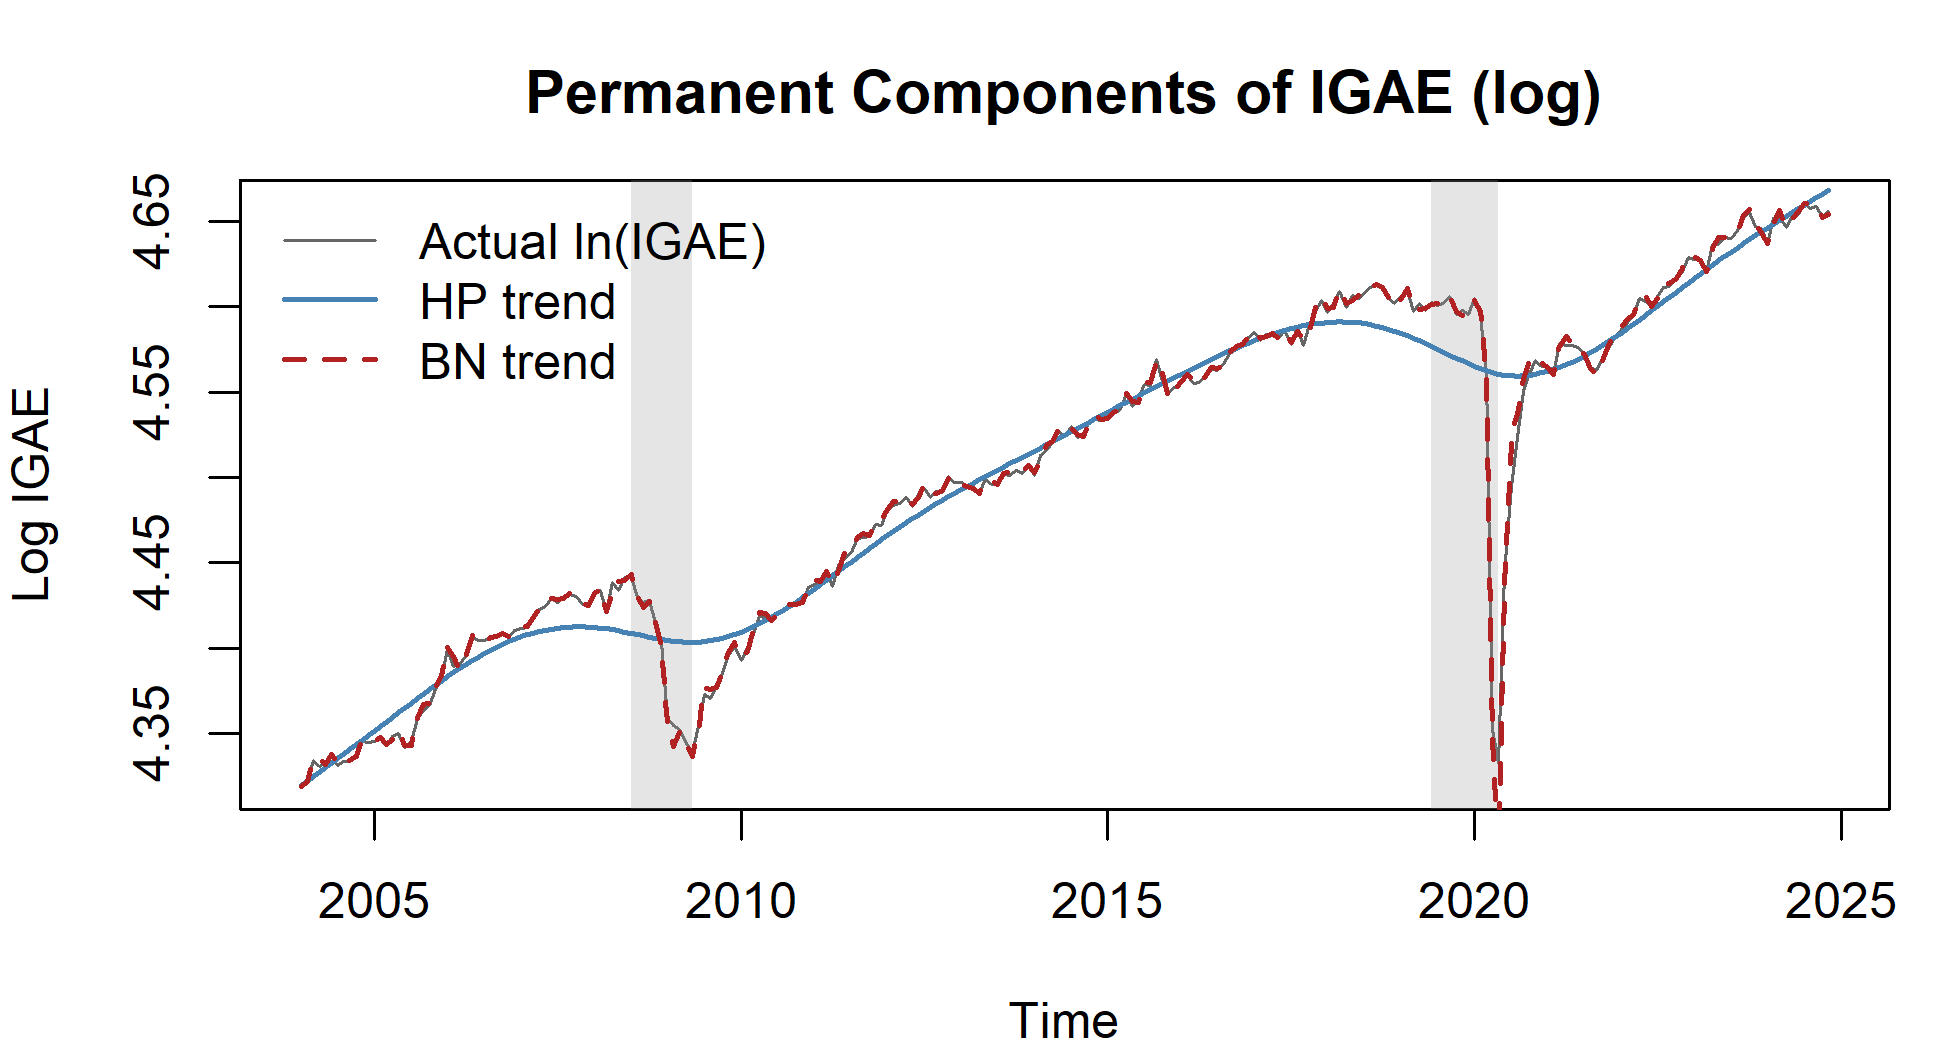
\includegraphics[width=\textwidth]{../ioae_assesment/outputs/eda/igae_trend.png}
\caption{IGAE estiamted trend components. HP filter using $\lambda= 1600$, BN using ARIMA(2,1,0) specification.}\label{fig:trend}
\end{figure}

\subsection{Multivariate analysis}\label{sec:multivariate}

The \cite{corona2022timely} panel time series consists of 27 variables used to nowcast IGAE on a timely basis, this panel has with the following characteristics: monthly frequency; starting from January 2004, with some available through January 2025; all variables have been obtained in seasonally adjusted form, or  if not, they have been adjusted using the X-13ARIMA-SEATS method\footnote{This seasonal adjustment relies on the automatic modeling procedure implemented in the \texttt{seas} function from R’s  \texttt{seasonal} package.}. The Table \ref{tab:all-dfm-vars} in Appendix shows the description of these variables and the transformation that is considered for the DFM.\footnote{I considered including the FFR adjusted for Zero-Lower Bound \citep{wu2016measuring}, the shadow federal funds rate to account; however, this series ends in early 2022. Similarly, the \cite{krippner2013measuring} (Reserve Bank New Zeland) alternative ends in September 2019 — leaving the COVID tightening cycle (2022–2025) unaddressed by either measure. I therefore exclude the FFR from the panel and note that US monetary policy transmission is partially captured through its effects on the exchange rate (TC), the Mexican short rate (TIIE-28), and the S\&P 500, all of which are already included.}


For each panel variable, optimal transformation is applied to each series with three possibilities: first-differences, monthly variation, yearly variation such that it maximizes the correlation with IGAE. This transformation is made for two purposes. First, to avoids having to incorporate the target variable into the DFM panel while preserving the economic relationship between the panel variables and economic activity, which is useful for forecasting purposes. Second, this transformation allows to account for the presence of deterministic trends and remove level shifts produced by any structural breaks, thus satisfying the $I(0)$ requirement and  to avoid spurious correlations in the DFM.  

One departure from \cite{corona2022timely} is done, the variables are classified into macro (21), and financial (6) variables. This taxonomy is done after the factors have been obtained, for the purposes of obtaining two uncertainty indexes under the methodology of \cite{jurado2015measuring}, not to perform a hierarchical DFM. The macroeconomic variables included in the analysis are presented in Figure \ref{fig:macro-dfm}, while the financial variables are shown in Figure \ref{fig:fin-dfm}.

\begin{figure}[H]
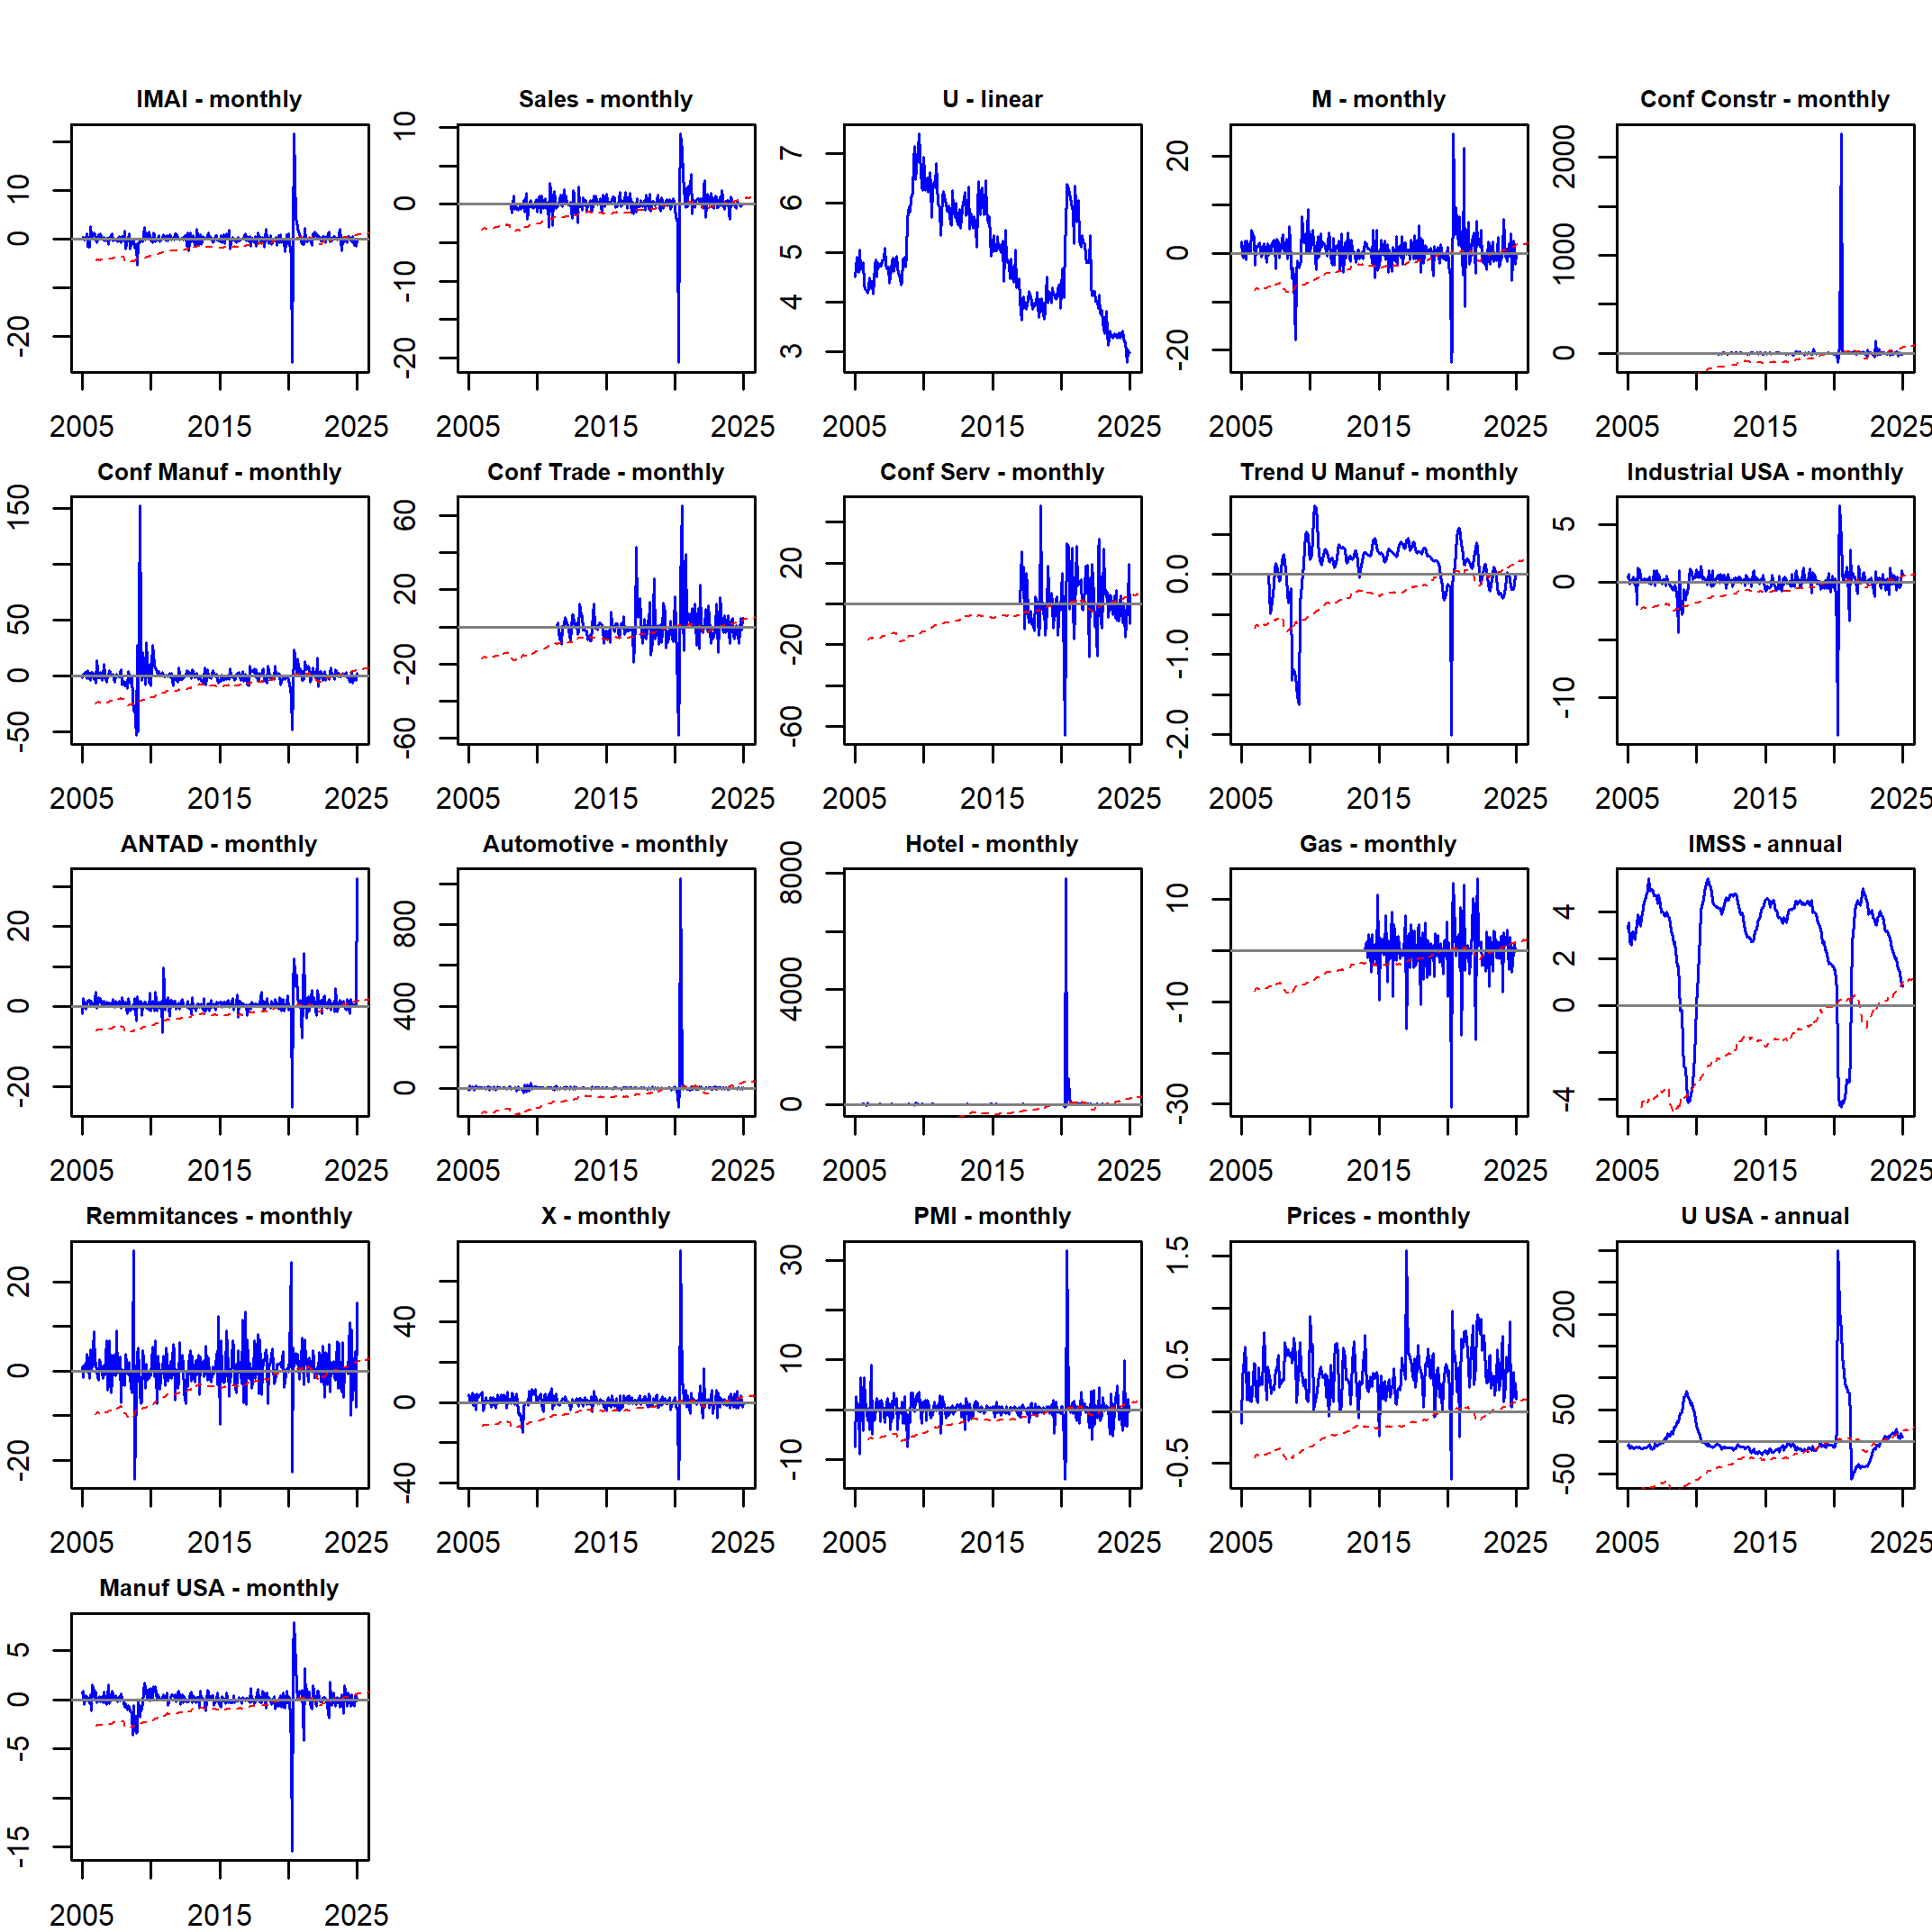
\includegraphics[width=\textwidth]{../ioae_assesment/outputs/eda/macro_dfm_vars.png}
\caption{Macroeconomic variables from \cite{corona2022timely}}\label{fig:macro-dfm}
\end{figure}

\begin{figure}[H]
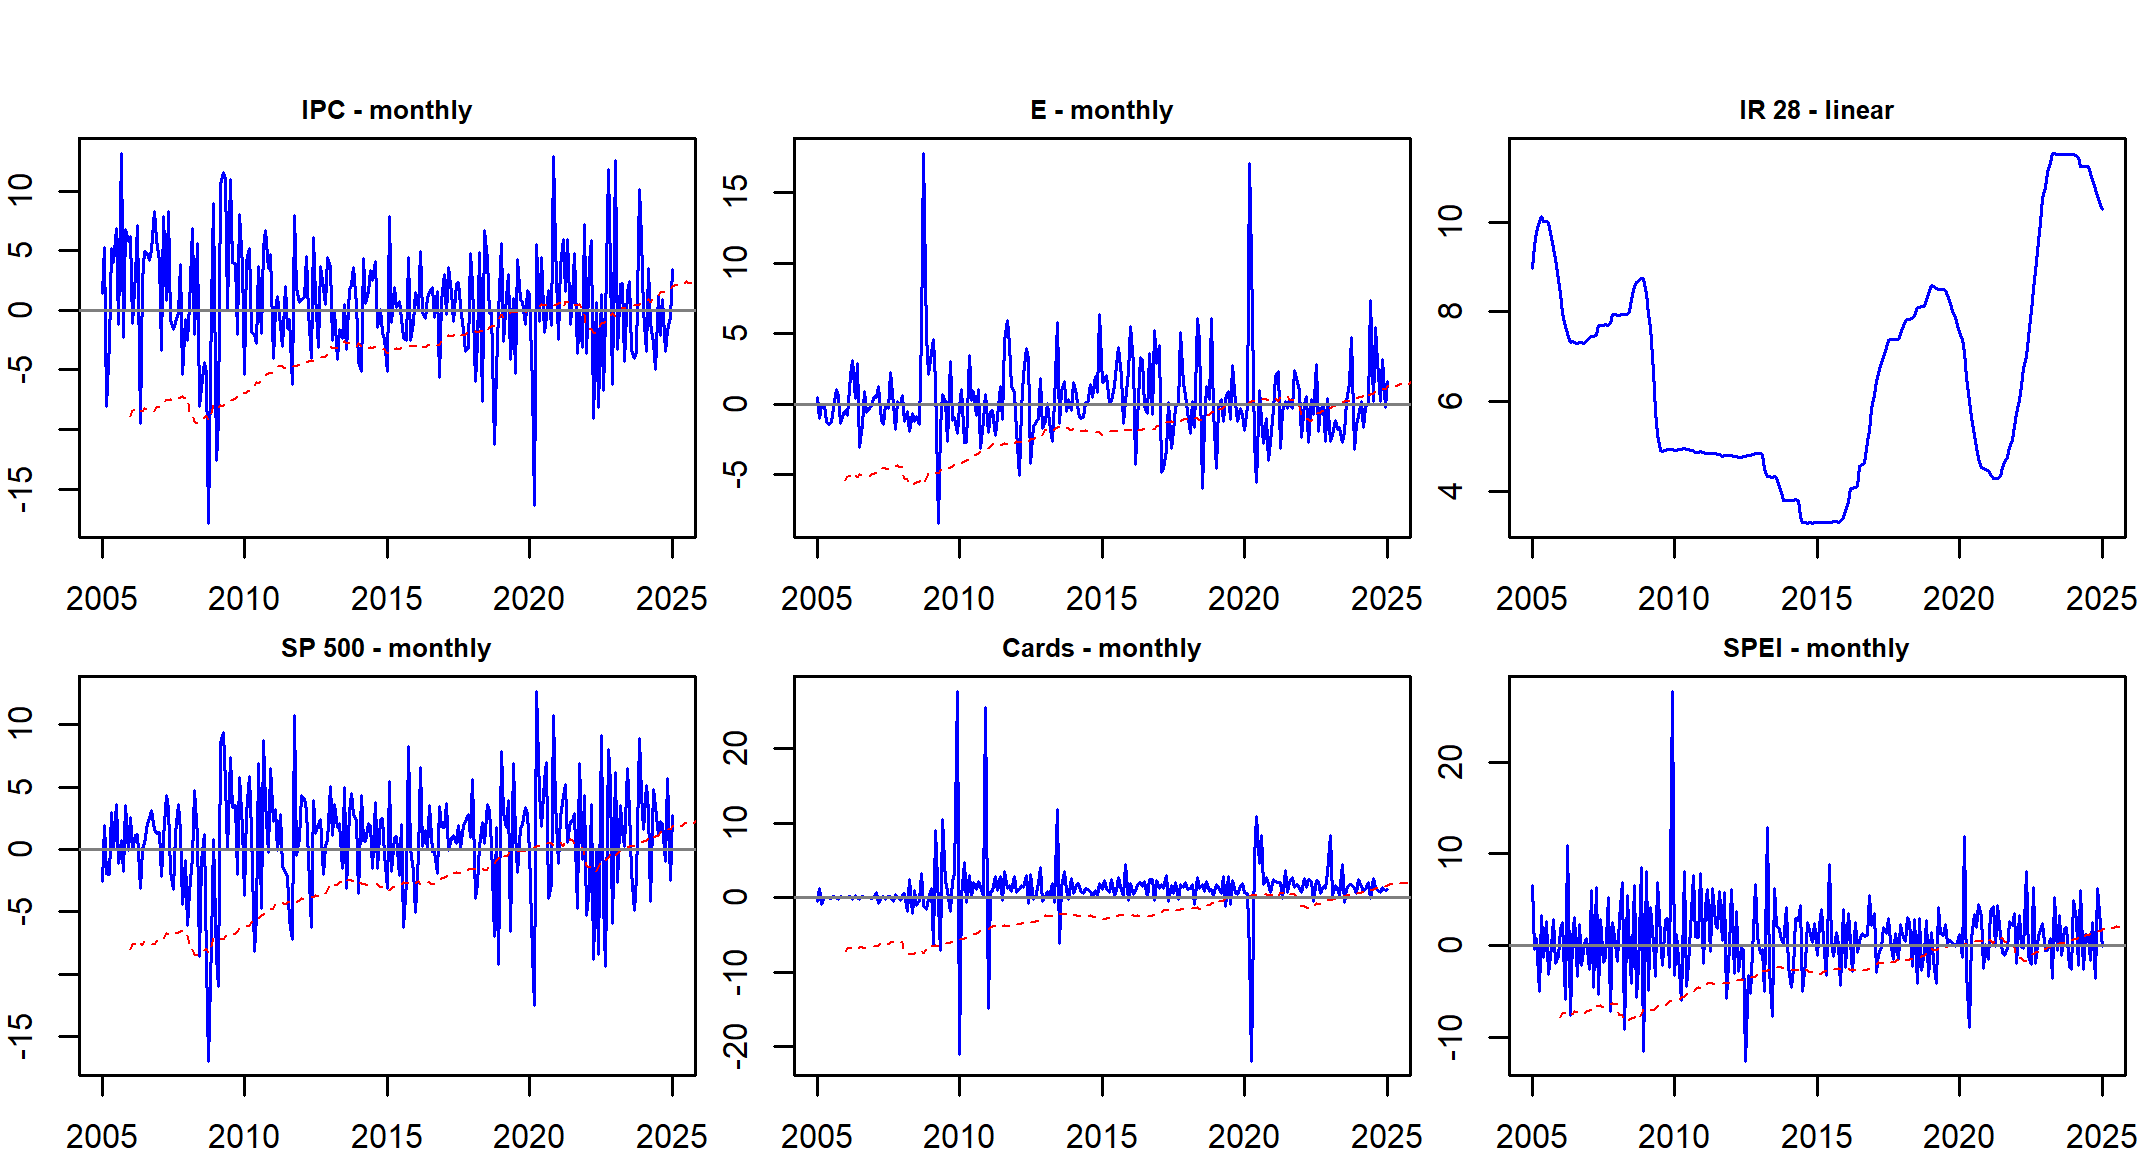
\includegraphics[width=\textwidth]{../ioae_assesment/outputs/eda/fin_dfm_vars.png}
\caption{Financial variables from \cite{corona2022timely}}\label{fig:fin-dfm}
\end{figure}








\section{Results}
\subsection{Dynamic Factor Model}\label{sec:DFM}

I first determine the number of factors using the \cite{bai2002determining} methodology, their three criteria minimize a penalized log-variance objective. The first criterion (IC1),includes $(N+T)/NT \cdot \ln(NT/(N+T))$, a penalty for a harmonic mean in $N$ and $T$ dimensions, the second criteria (IC2), includes $(N+T)/NT \cdot \ln(\min(N,T))$, which imposes a higher penalty when either dimension is small, while the third criteria (IC3),$\ln(\min(N,T))/\min(N,T)$, grows relatively slowly with the panel size and therefore tends to over-select factors. The results are shown in Table~\ref{tab:bai-ng-crit}: IC1 and IC2 select $r = 7$, whilst IC3 suggests $r = 8$. I decide to take 7, by majority of criteria. The seven factors explain 66.9\% of total panel variance, while the the remaining 33.1\% is idiosyncratic variance, and is to be used for the GARCH modeling under the JLN methodology. 



\begin{table}[h]
\centering
\begin{threeparttable}
\caption{Determining the number of factors Bai \& Ng (2002) criteria}\label{tab:bai-ng-crit}
\begin{tabular}{crrrr}
\hline
$r$ & \textbf{IC1} & \textbf{IC2} & \textbf{IC3} \\
\hline
0 & $-0.004$ & $-0.004$ & $-0.004$ \\
1 & $-0.191$ & $-0.186$ & $-0.200$ \\
2 & $-0.200$ & $-0.192$ & $-0.219$ \\
3 & $-0.205$ & $-0.192$ & $-0.233$ \\
4 & $-0.208$ & $-0.190$ & $-0.245$ \\
5 & $-0.215$ & $-0.193$ & $-0.262$ \\
6 & $-0.218$ & $-0.192$ & $-0.274$ \\
\textbf{7} & $\mathbf{-0.233}$ & $\mathbf{-0.202}$ & $-0.298$ \\
\textbf{8} & $-0.228$ & $-0.193$ & $\mathbf{-0.302}$ \\
\hline
\end{tabular}
\begin{tablenotes}
    \small
    \item \textit{Notes:} Information criteria to determine the optimal number of common latent factors ($r$) to extract from the macroeconomic panel data used for constructing the financial indices. Bold values indicate the minimum value achieved by each respective criterion, identifying the optimal factor allocation. %IC\_p1, IC\_p2, and IC\_p3 denote the three alternative panel information criteria specifications, each employing a distinct penalty function for overparameterization based on both the cross-sectional dimension ($N$) and the time series length ($T$). Bold values indicate the minimum value achieved by each respective criterion, identifying the optimal factor allocation. While IC\_p1 and IC\_p2 minimize at $r=7$, IC\_p3 selects $r=8$. The more parsimonious choice of seven common factors is selected for the baseline specification to ensure stable structural dynamics.
\end{tablenotes}
\end{threeparttable}
\end{table}



In addition, Figure~\ref{fig:loadings} show the factor loadings that allow for interpretation of the results. We see that the first factor, F1, is mostly related to activities in the transformation sectors in the economy both for the Mexican and the US economy: industrial production, manufacturing, automobile production, exports and imports, we can even refer to it as the Mexican business cycle. The second factor, F2,  is mainly related to unemployment both in Mexico and in the US, and stock markets, also in both countries, also it is negatively correlated to the level of formal employment registration in Mexico, IMSS; this can be called as labor market stress $+$ equity markets. The third factor, F3, relates the most to exchange rate, US unemployment and remittances, while at the same time negatively related to stock markets, employment in the manufacturing industry and the formal employment registry, IMSS; this factor captures the effect of peso depreciation and remittances. The fourth factor, F4, considers mainly the statisitcal relationship to the interest rate and negatively related to the unemployment rate; clearly reflects monetary policy and interest rate channel. The fifth one, F5, is associated with lodging services, $Hotel$, but negatiely related to automobile production, manufacturing, exports and imports; this factor mostly reveals the relation between domestic sector versus  external manufacturing factor. The sixth factor, F6, is negatively related to banking information, cards and SPEI, and in lesser amount to manufacturing confidence; this factor accounts for credit and financial conditions. Finally, the seventh factor, F7, is related to business and consumer sentiment, with confidence indexes for consumers, commerce, services, and manufacturing all loading positively.


\begin{figure}[H]
\centering
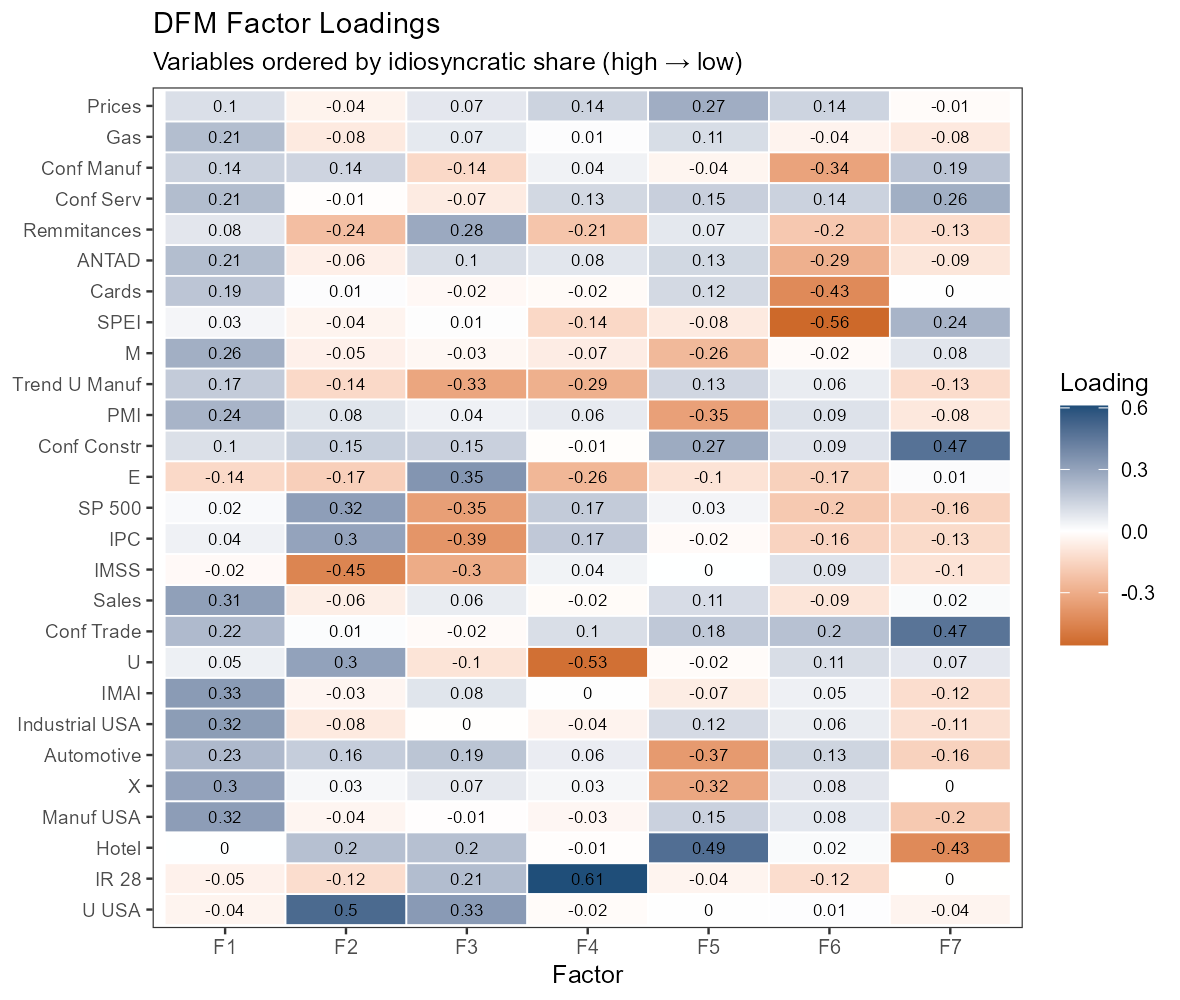
\includegraphics[width=\textwidth]{../ioae_assesment/outputs/lmn/fig8_loadings_heatmap.png}
\caption{DFM factor loadings}\label{fig:loadings}
\end{figure}


Given these interpretation to the seven estimated factors, in Figure~\ref{fig:factors} I show the evolution of them. Note that three of them ---F1 - business cycle, F5 - domestic vs external sector, F7 - business and consumer sentiment--- vary alongside the dynamic of IGAE monthly variations shown in the bottom of Figure \ref{fig:igae_panels}. The factors F2 and F3 clearly capture the large swings during the recessions commented before, the Great Recession and COVID-19 pandemic, consistent with the simultaneous rise in unemployment and currency pressure during both episodes. The factor F4, 
Notably, F6 - credit and financial conditions, is the only one that do not reflects the large falls during recessions, and captures persistent background
volatility throughout the sample given that it does not capture the large tail events.



\begin{figure}[H]
\centering
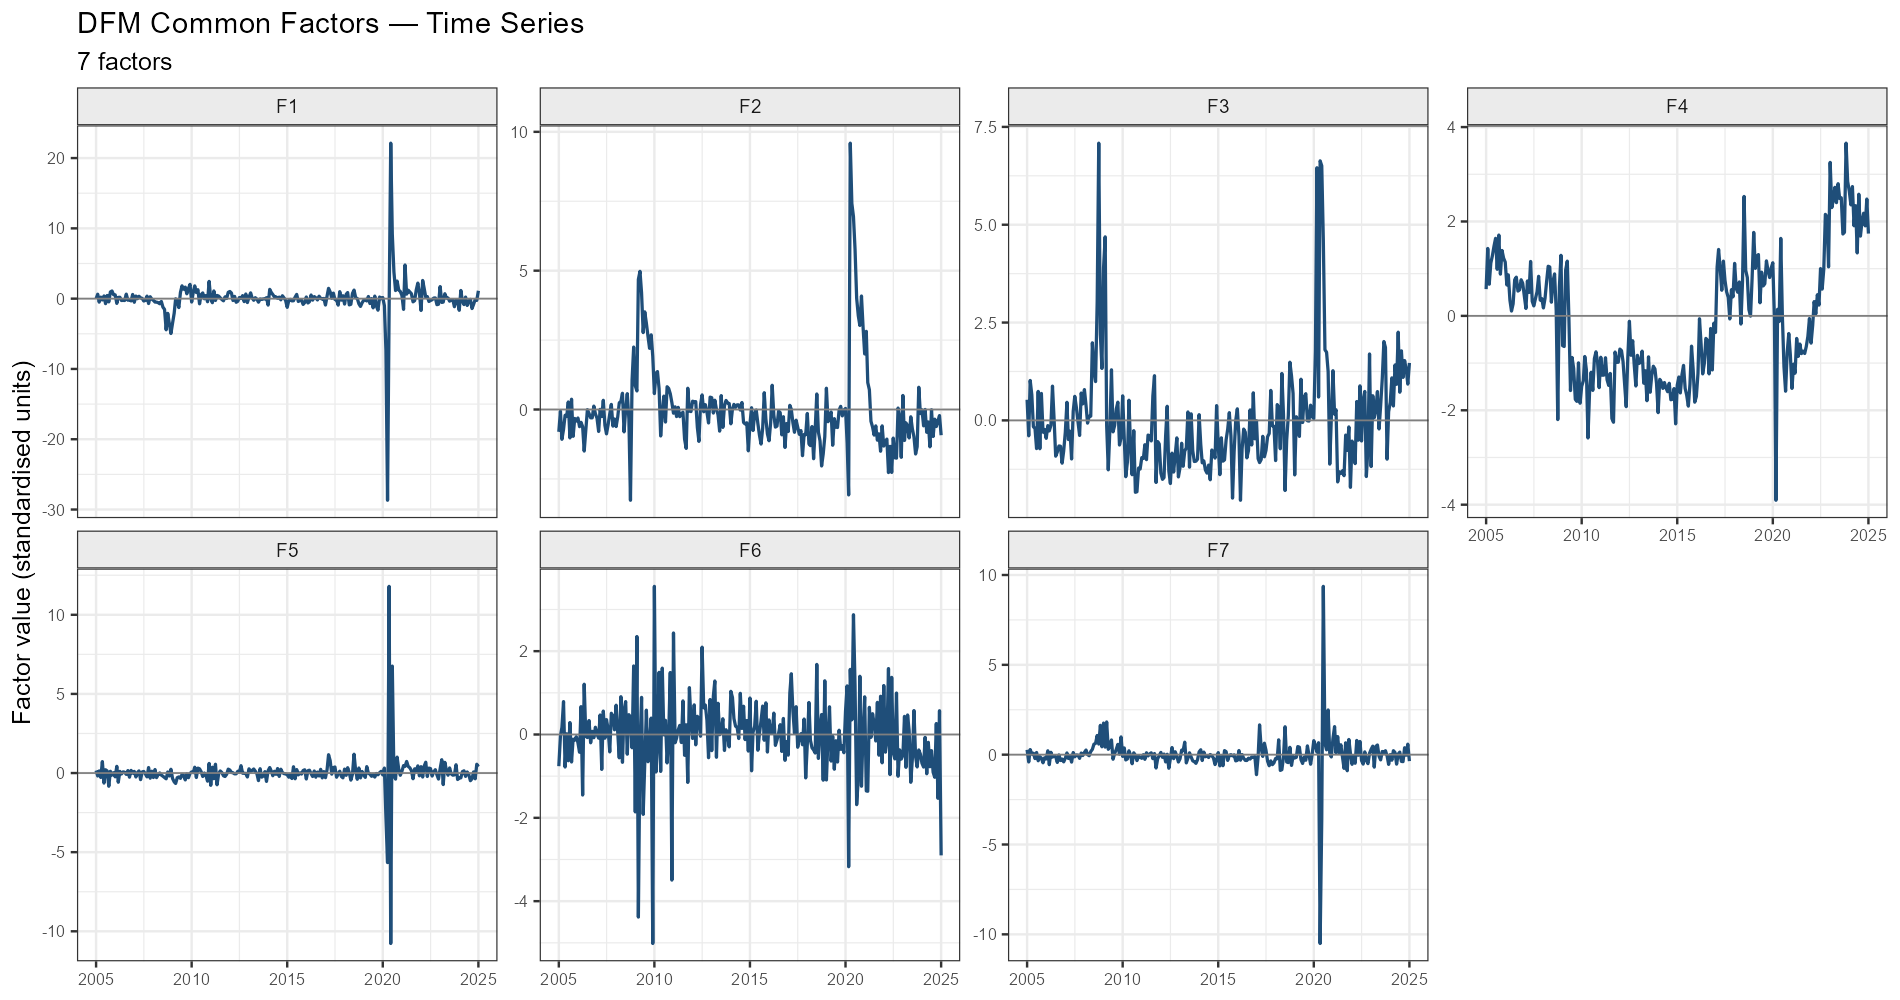
\includegraphics[width=\textwidth]{../ioae_assesment/outputs/lmn/fig7_factors_ts.png}
\caption{Factors extracted for the 27 variables panel for the Mexican economy}\label{fig:factors}
\end{figure}



\subsection{Macroeconomic and Financial Uncertainty}\label{sec:MU-FU}

Once the DFM have been estimated, the idiosyncratic component for variable $i$ at time $t$ is obtained as a residual, which are later aggregated into uncertainty measures for the macroeconomic conditions and the financial conditions of the Mexican economy. Figure~\ref{fig:MU-FU} shows these estimations along with the monthly variations of IGAE. 


\begin{figure}[H]
\centering
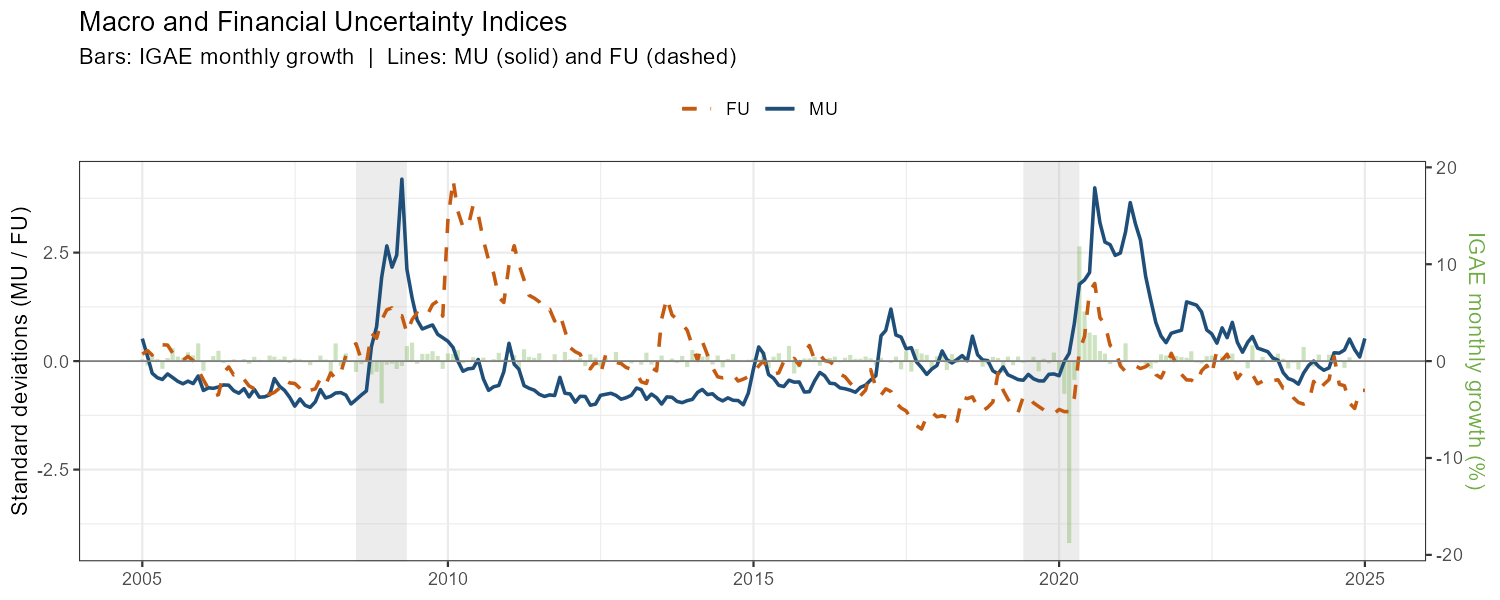
\includegraphics[width=\textwidth]{../ioae_assesment/outputs/lmn/fig1_mu_fu_indices.png}
\caption{Macroeconomic and Financial Uncertainty indexes for  the Mexican economy}\label{fig:MU-FU}
\end{figure}


By construction, the uncertainty indicators capture the unforeseeable component of the macroeconomy and financial conditions. Both indices are standarized, thus
values below zero indicate uncertainty is below its historical averages; values above indicate high uncertainty episodes. 

MU indicator remains in general near or below zero throughout most sample, consistent with Mexico's relatively stable macro conditions in the period inter-crisis (2010-2018). Some exceptions are the spikes around the begining of the GFC and modest upward react to political turmoil eents as the 2012 and 2018 Mexican elections and the 2016 US elections. The post COVID pandemic recession, shows that this indicator has been on positive terrain, indicating a period of relative higher macroeconomic uncertainty.

In the case of FU, we see that this indicator reacted earlier in the GFC, but its spike was not during the main period of recession, but during the recovery part around 2009-2010. Similarly, this indicator increased around 2013-2014 on its own, while the MU remained on its regular level below zero. In addition, after the COVID-19 episode, the FU indicator, increased but returned very quickly and have remained below the zero afterwards. This divergence suggests that financial markets priced in and resolved the COVID uncertainty relatively fast, while real macroeconomic conditions remained structurally less predictable.

As a benchmark comparison, in Figure~\ref{fig:EPU} I compare the MU and FU indices to the one available for the Mexican economy under the \cite{baker2016measuring} methodology. The EPU is mostly related to the MU than to the FU; note, however, that the EPU is text-based and reacts to news flow, while MU measures realized unpredictability in macro data, which took longer to subside. In particular, both spike sharply and simultaneously at the begining of GFC (2008); similarly, both spike and both remain elevated in the post-pandemic period through 2022–2024; during the period 2017–2018, both show a moderate rise, consistent with NAFTA renegotiation uncertainty and the 2018 Mexican election; finally, in recent times both turning upward, consistent with US tariff and trade policy uncertainty. 

\begin{figure}[H]
\centering
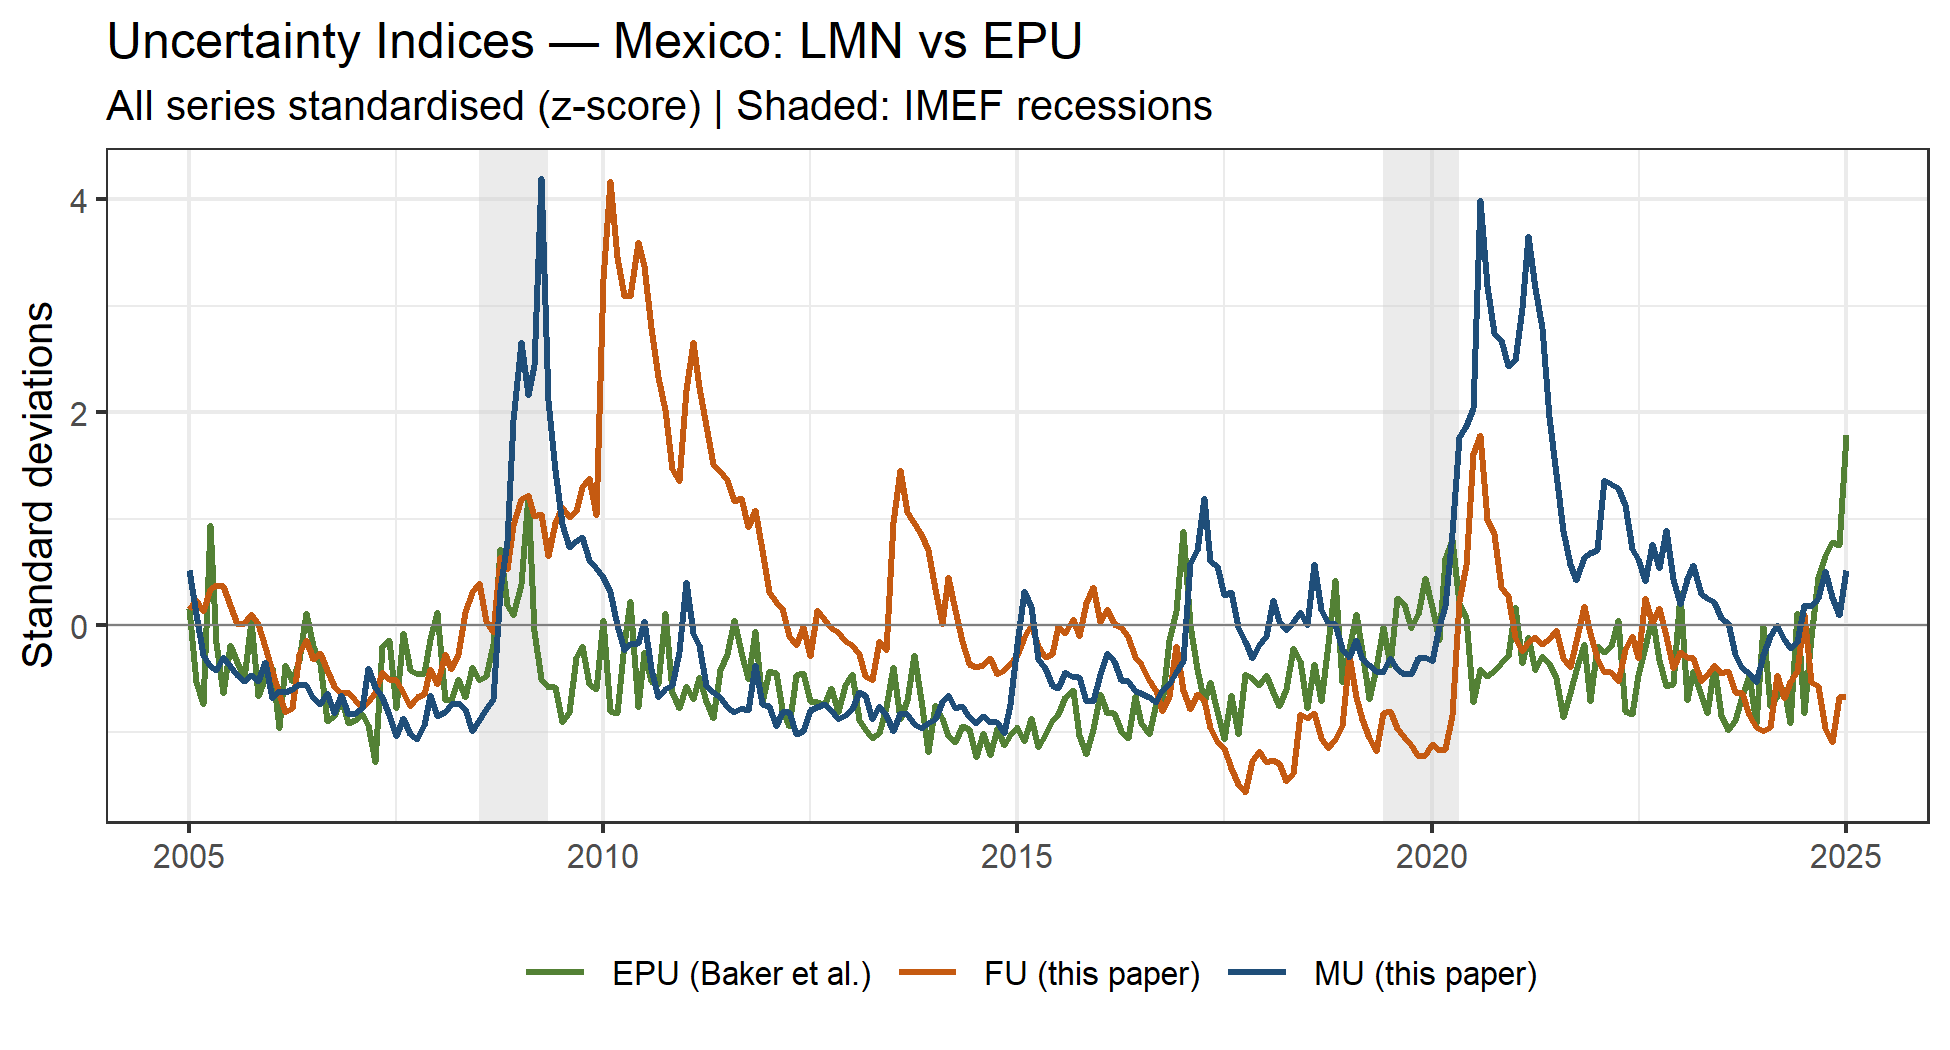
\includegraphics[width=\textwidth]{../ioae_assesment/outputs/lmn/fig_epu_compare.png}
\caption{Comparison with the Mexican EPU under Baker et al. (2016) methodology.}\label{fig:EPU}
\end{figure}




\subsection{VAR estimation}\label{sec:SVAR}

The VAR estimation is performed in accordance to \cite{ludvigson2021uncertainty} framework in which the Cholesky ordering of variables is MU $\rightarrow$ IGAE $\rightarrow$ FU (A: MU first). Similarly, an alternative VAR ordering is tested, in which the FU precedes IGAE and MU, respectively (B: FU first). The baseline analysis is conducted with specification A, and then the model is estimated with B specification for comparison. 


To proceed with VAR estimation, I first added the impulse-type dummies from the exogenous and endogenous tests in section \ref{sec:structural-breaks}. Then, to select the appropriate number of lags I compare three different information criteria: Akaike (AIC), Hannan and Quinn (HQ) and Schwarz (SC). The results from these tests are presented in Table~\ref{tab:lag-select}:  AIC selects $p = 5$, HQ selects $p = 2$, and SC selects $p = 1$. Note that, with $p = 1$ and $K = 3$ variables the VAR has $K \times (K + 1) = 12$ free parameters; thus, I use as the baseline for parsimony I use $p =1$. 

\begin{table}[H]
\centering
\caption{Lag selection with different information criteria}\label{tab:lag-select}
\begin{tabular}{cccc}
\hline
$p$ & \textbf{AIC} & \textbf{HQ} & \textbf{SC}  \\
\hline
1 & $-3.54$ & $-3.44$ & $\mathbf{-3.28}$ \\
2 & $-3.65$ & $\mathbf{-3.48}$ & $-3.25$ \\
3 & $-3.61$ & $-3.40$ & $-3.08$ \\
4 & $-3.71$ & $-3.44$ & $-3.04$ \\
5 & $\mathbf{-3.76}$ & $-3.43$ & $-2.95$ \\
6 & $-3.73$ & $-3.35$ & $-2.79$ \\
\hline
\multicolumn{4}{l}{%
 \parbox{0.5\textwidth}{\footnotesize \textit{Notes:} Bold indicates the
  selected lag for each criterion. VAR model:
  $\mathbf{X}_t = (MU_t,\, IGAE_t,\, FU_t)'$, $p_{\max} = 6$.
  Impulse dummies for 2009/05 and 2020/04 included as exogenous regressors.
  Baseline uses $p = 1$ (SC); robustness at $p = 5$ (AIC).}} \\
\end{tabular}
\end{table}

In addition, I perform likelihood ratio tests to determine wheter additional lags improve the model. The LR test compares a restricted VAR($p_r$) against an unrestricted VAR($p_u$), with null hypothesis that the additional coefficients matrices are jointly zero --- the restricted model fits as well as the unrestricted one. The results presented in \ref{tab:lr-tests} show that adding lag 2 over lag 1 is statistically significant ($p$), but lag 3 does not add with respect to lag 2. Lag 4 then re-enters significantly (LR $= 41.16$ over $p=3$, $p < 0.001$), and the joint test $p=1$ vs $p=4$ strongly rejects parsimony (LR $= 92.18$, $p < 0.001$). Thus, although SC selects $p = 1$, the joint rejection of $p = 1$ against $p = 4$ (LR $= 92.18$, $p < 0.001$) and the richer impulse response dynamics at $p = 4$ shown in next section lead me to adopt $p = 4$ as the baseline specification; $p = 1$ is retained as a parsimony robustness check.


\begin{table}[H]
\centering
\caption{Likelihood ratio tests for VAR lag order}\label{tab:lr-tests}
\begin{tabular}{llrrc}
\hline
$H_0$ & $H_1$ & LR stat & df & $p$-value \\
\hline
$p = 1$ & $p = 2$ & $41.86$ & $9$  & $0.000^{***}$ \\
$p = 2$ & $p = 3$ &  $9.75$ & $9$  & $0.371$       \\
$p = 3$ & $p = 4$ & $41.16$ & $9$  & $0.000^{***}$ \\
$p = 3$ & $p = 5$ & $69.06$ & $18$ & $0.000^{***}$ \\
$p = 1$ & $p = 4$ & $92.18$ & $27$ & $0.000^{***}$ \\
\hline
\multicolumn{5}{l}{%
  \parbox{0.72\textwidth}{\footnotesize \textit{Notes:}
  LR $= T(\ln|\hat{\Sigma}_r| - \ln|\hat{\Sigma}_u|) \sim \chi^2(K^2 \Delta p)$,
  where $K = 3$. All models estimated on a common sample (rows $p_{\max}+1$ to $T$)
  with dummies for 2009/05 and 2020/04 included as exogenous regressors.
  $^{***}$ $p < 0.01$.}} \\
\end{tabular}
\end{table}


Results for VAR estimation are shown in Figure ~\ref{fig:VAR} at $p=4$. Top panel, \ref{fig:IRF-MU}, shows impulse response functions for both specifications; irrespective of ordering, the two plots show that neither uncertainty channel produces a statistically significant response of IGAE growth at any horizon: zero lies within the 90\% bootstrap bands throughout both panels. Under ordering A, a
one-standard-deviation MU shock reveals a small negative impact on IGAE that recovers around months 4--5, consistent
with a wait-and-see mechanism, as in the literature of the EPU; in addition, the FU shock produces a
positive impact response under both orderings, which is counterintuitive. Under ordering B, responses are similar in direction but with different magnitude. MU responses are
stable across orderings, while FU responses are larger in Panel B, indicating that that FU's influence on IGAE operates primarily within the same month
and is suppressed by the Cholesky restriction when FU is ordered last.


The bottom panel, \ref{fig:FEVD}, shows the forecast variance error decomposition for both specifications. In any case, IGAE own dynamics account for more than 98\% of the FEVD, leaving less than 2\% to the uncertainty indicators. MU contributes approximately 0.8\% at the 24-month horizon and is insensitive to ordering. FU is ordering-sensitive: its share is approximately 0.65\% under Ordering A but rises
to approximately 1.35\% under Ordering B.


\begin{figure}[htbp]
\centering
\begin{subfigure}[b]{\textwidth}
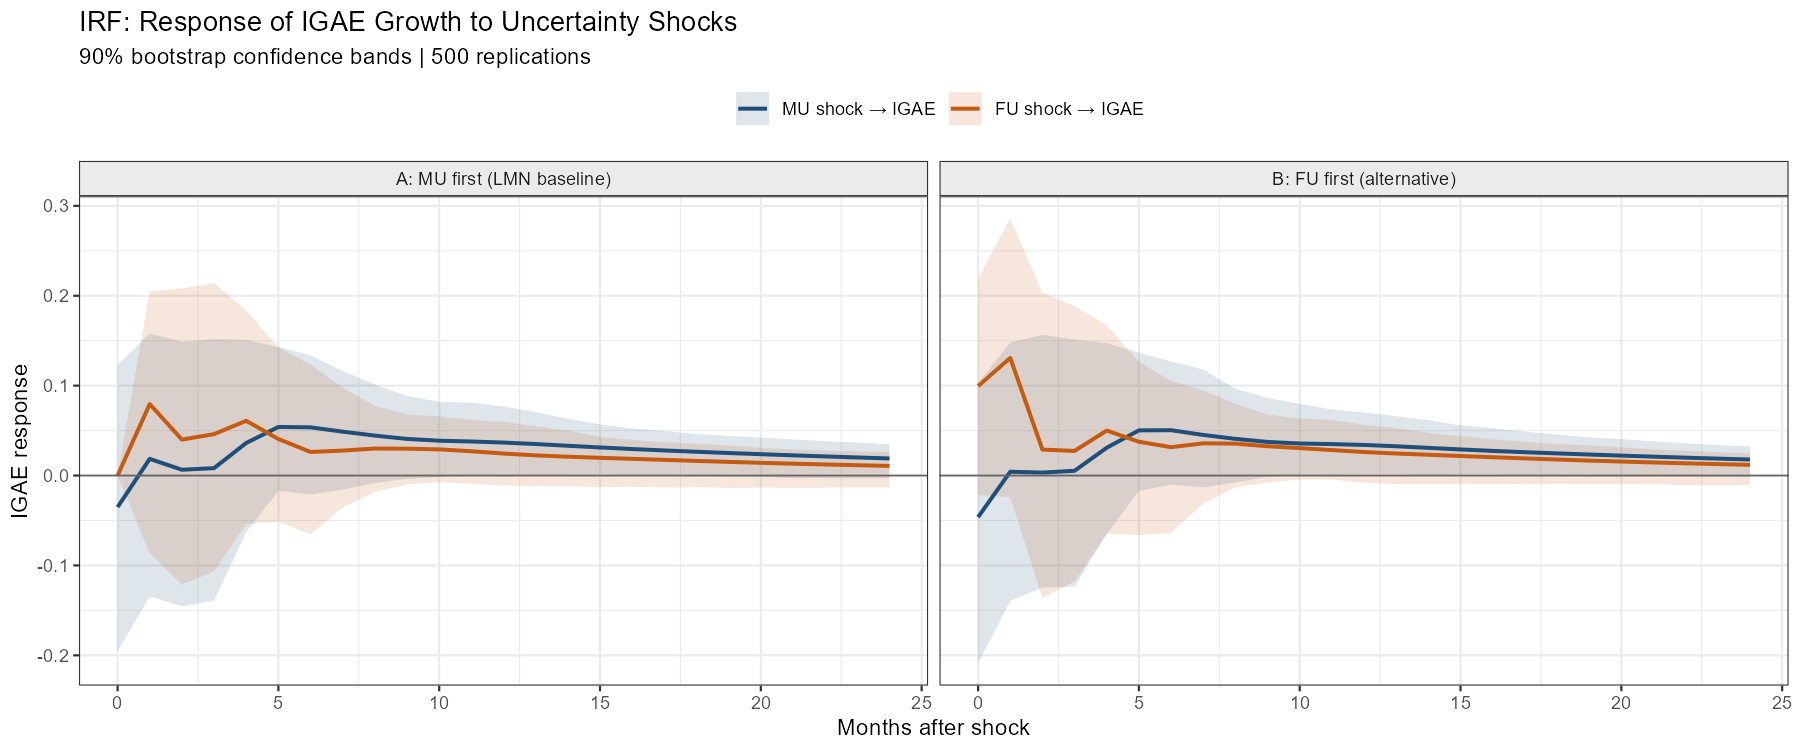
\includegraphics[width=\textwidth]{../ioae_assesment/outputs/lmn/fig4_irfs_p4.png}
\caption{Impulse Response Function}\label{fig:IRF-MU}
\end{subfigure}
  \vspace{4mm}
\begin{subfigure}[b]{\textwidth}
\centering
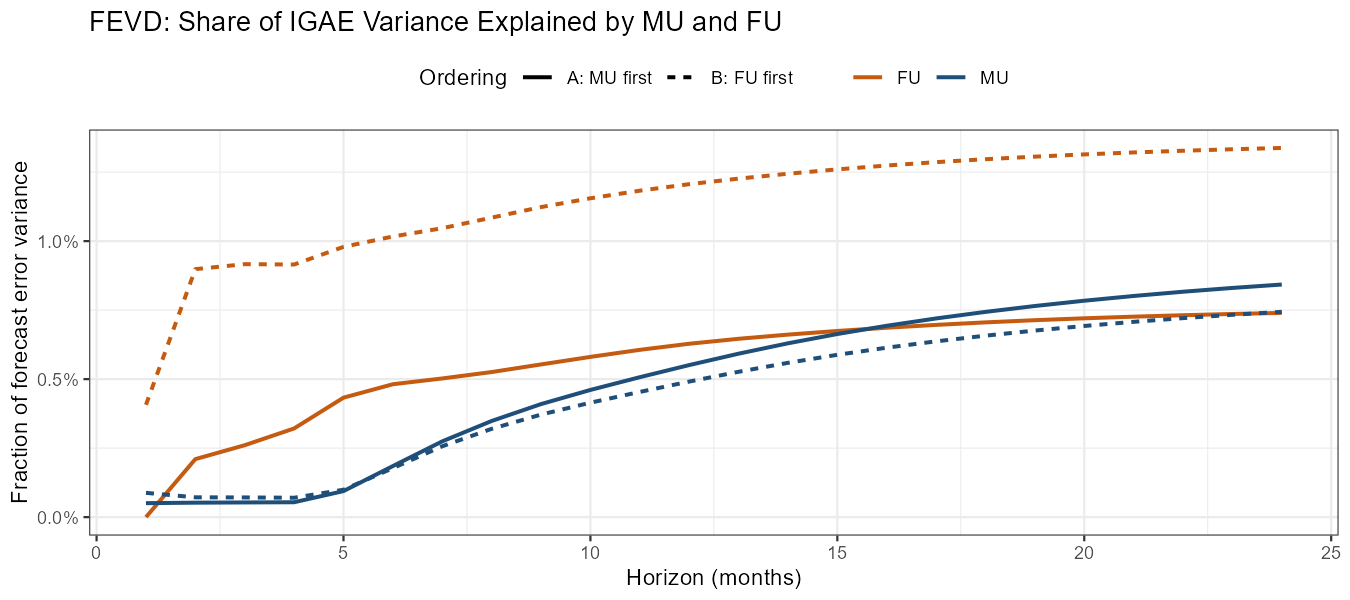
\includegraphics[width=.8\textwidth]{../ioae_assesment/outputs/lmn/fig5_fevd_p4.png}
\caption{Forecast Error Variance Decomposition}\label{fig:FEVD}
\end{subfigure}
\caption{VAR estimation. Variables included MU $\rightarrow$ IGAE $\rightarrow$ FU}\label{fig:VAR}
\end{figure}

\subsection{Local Projection}\label{sec:LP}
As a robustness check, I estimate IRF under the approach of \cite{jorda2005estimation}. This methodology rather than recovering IRFs from the VAR's recursive structure, uses the orthogonal shocks of the VAR model to compute the response at each horizon, by projecting the outcome $h$ periods ahead on the structural shock today. 

In this case the estimated equation at each horizon $h = 0, 1, \ldots, 24$ is:

$$IGAE_{t+h} = \alpha_h + \beta^{MU}_h \cdot \varepsilon^{MU}_t + \beta^{FU}_h \cdot \varepsilon^{FU}_t + \sum_{j=1}^{p} \boldsymbol{\gamma}^{\prime}_{h,j}\,
                \mathbf{X}_{t-j} + e_{t+h}$$

\noindent where $\mathbf{X}_{t-j} = (MU_{t-j},\, IGAE_{t-j},\, FU_{t-j})'$ are $p = 4$ lags of the VAR variables included as controls. As seen in Figure~\ref{fig:LP}, the results do not vary significantly from the obtained above: point estimates are close to zero at all horizons and statistically insignificant throughout.

\begin{figure}[H]
\centering
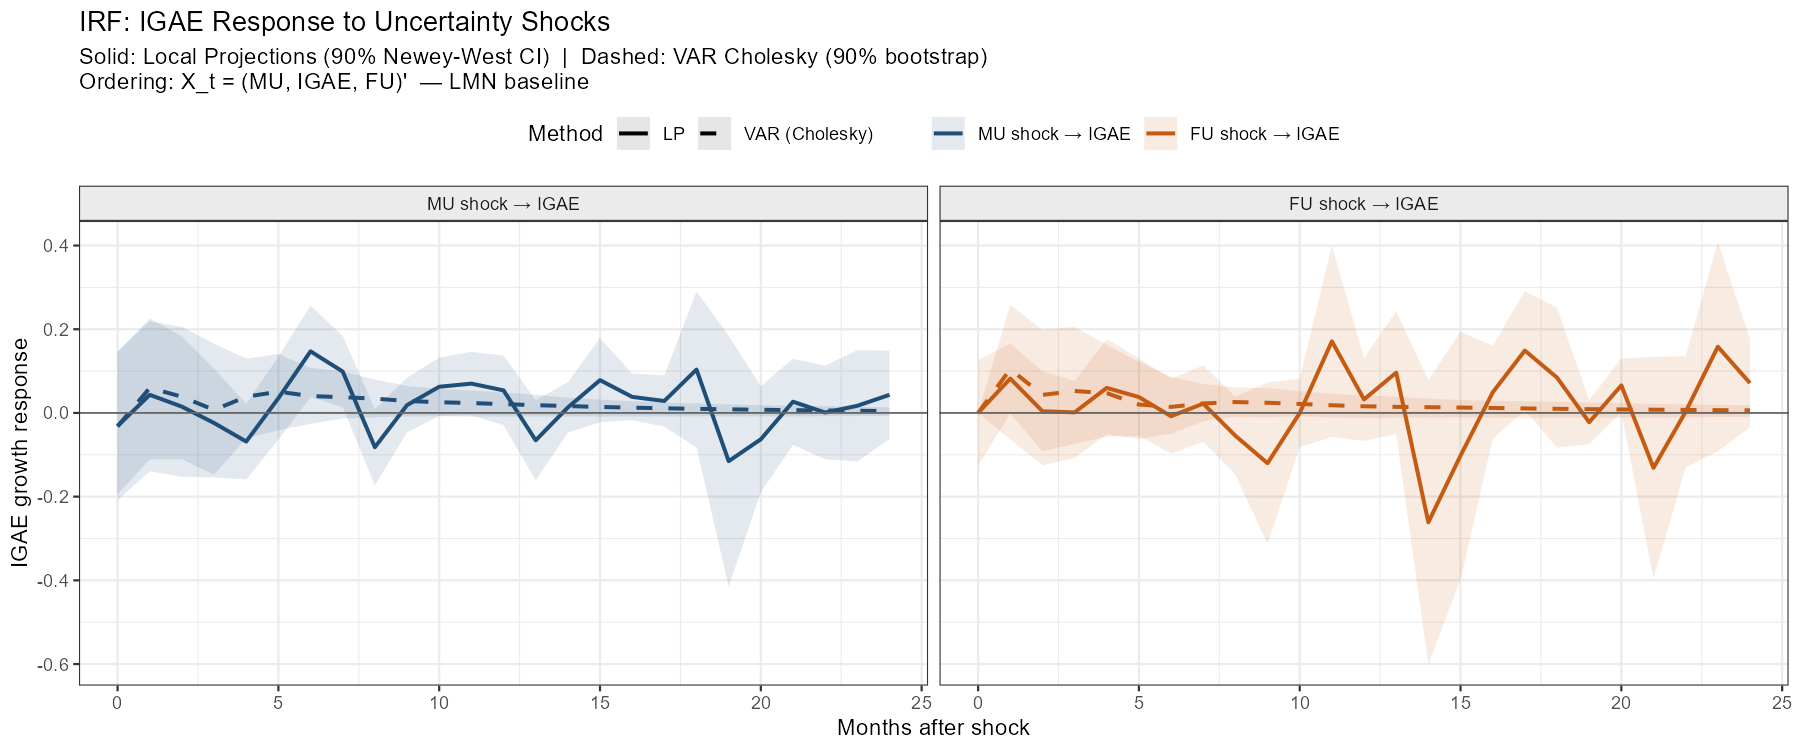
\includegraphics[width=\textwidth]{../ioae_assesment/outputs/lmn/fig6_lp_irf.png}
\caption{IRF estimated with Local Projections methodology}\label{fig:LP}
\end{figure}




\subsection{Growth-at-Risk}\label{sec:GaR}

Once I have constructed the uncertainty indicators, MU and FU, I can incorporate them into the \cite{adrian2019vulnerable} framework to assess their relevance into the forecast of IGAE growth conditional on current conditions and uncertainty. 




The results of these quantile regressions are presented in Figure~\ref{fig:gar_all} for $h \in \{1, 3, 6, 12\}$ months. Three features are consistent across all
horizons. First, the GaR estimate (5th percentile, red) lies persistently
below zero even in periods of no stress, this reveals that downside risk is always present, not only
during recessions. Second, both the GFC and the COVID-19 recession are
captured by sharp deteriorations in the lower tail, confirming that
 MU and FU have predictive content for extreme negative growth
outcomes. Third, the range between the 5th and 95th percentile widens substantially with the horizon; at $h=1$ the uncertainty conditions
contain most of the near-term distributional information, and expands at $h = 12$, reflecting genuine uncertainty about growth a year
ahead.


In addition, the horizon dimension also reveals  important asymmetries. At $h = 1$, the GaR is near zero in tranquil periods and collapses to approximately
$-24\%$ during COVID. At $h = 12$, the GaR is persistently around $-7$\,to\,$-9\%$ throughout the sample, including in expansion phases,
and the 95th percentile expands to $+25\%$ during the post-GFC recovery ---
indicating that a year-ahead outlook carries both large downside and
large upside risk. 



\begin{figure}[htbp]
  \centering

  \begin{subfigure}[b]{0.48\textwidth}
    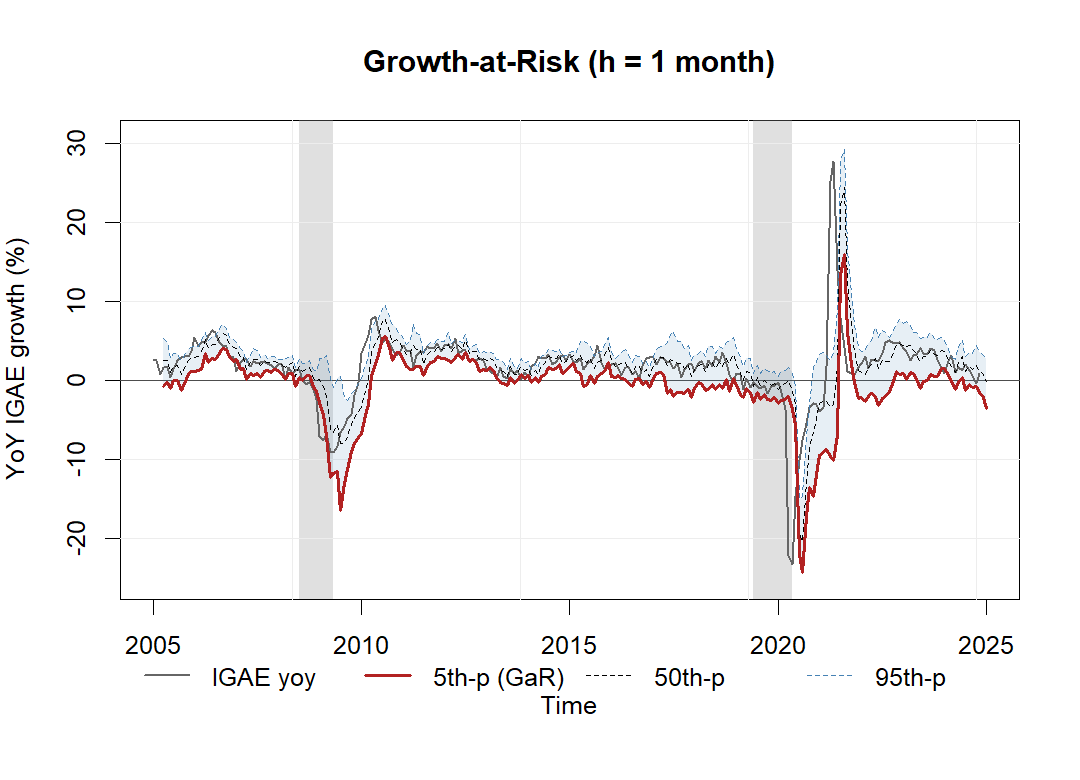
\includegraphics[width=\textwidth]{../ioae_assesment/outputs/abg/fan_plot_h1.png}
    \caption{$h = 1$ month}
    \label{fig:gar_h1}
  \end{subfigure}
  \hfill
  \begin{subfigure}[b]{0.48\textwidth}
    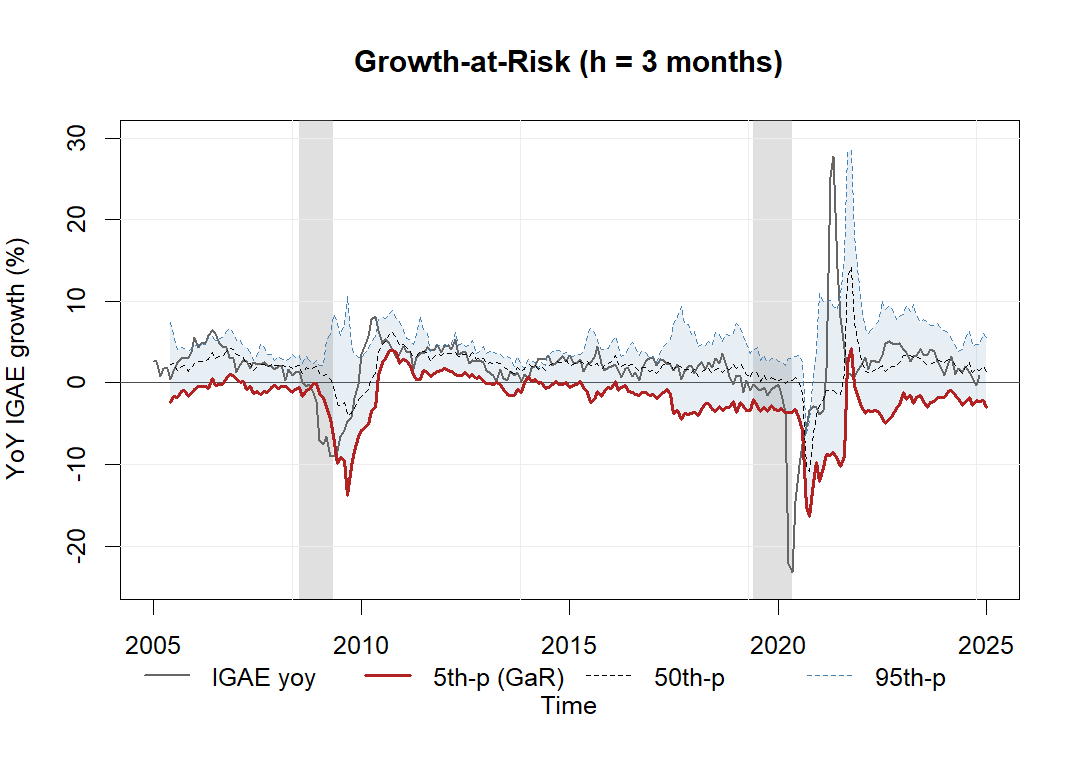
\includegraphics[width=\textwidth]{../ioae_assesment/outputs/abg/fan_plot_h3.png}
    \caption{$h = 3$ months}
    \label{fig:gar_h3}
  \end{subfigure}

  \vspace{4mm}

  \begin{subfigure}[b]{0.48\textwidth}
    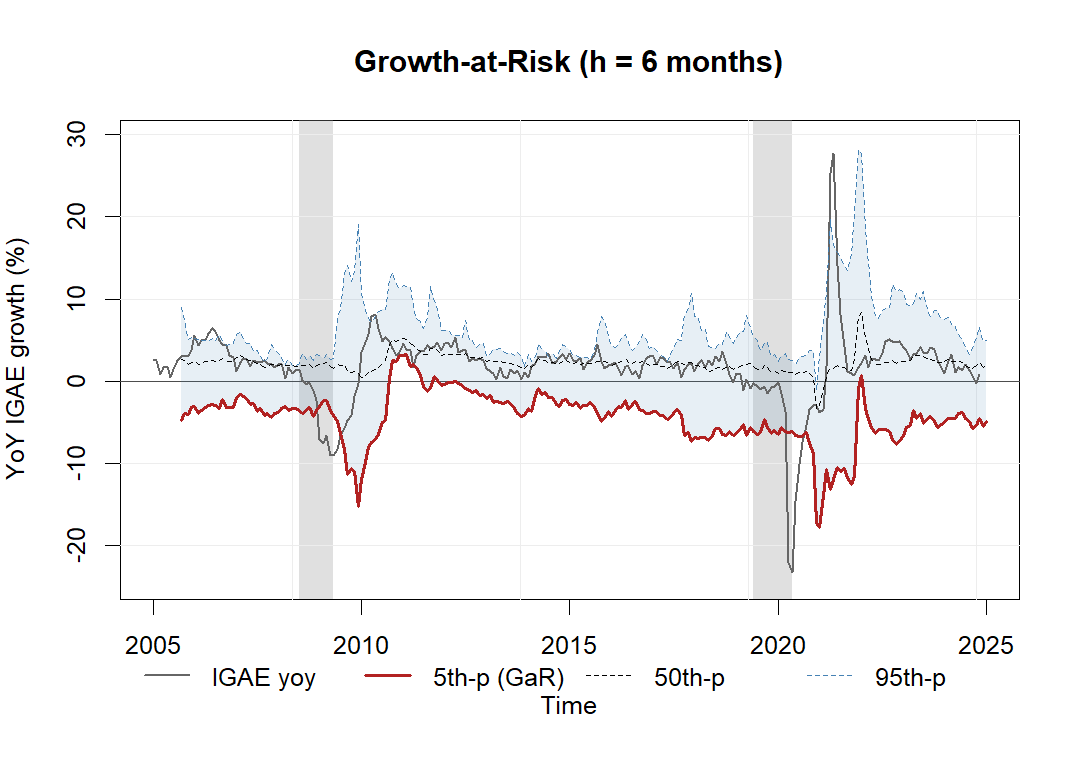
\includegraphics[width=\textwidth]{../ioae_assesment/outputs/abg/fan_plot_h6.png}
    \caption{$h = 6$ months}
    \label{fig:gar_h6}
  \end{subfigure}
  \hfill
  \begin{subfigure}[b]{0.48\textwidth}
    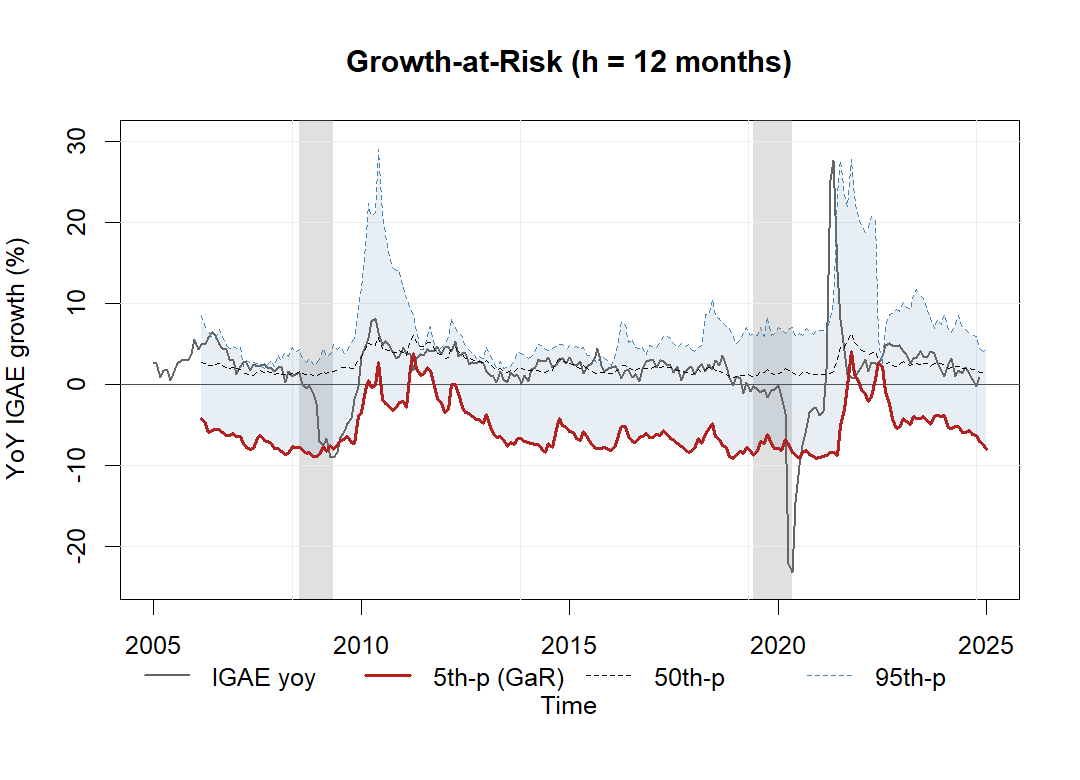
\includegraphics[width=\textwidth]{../ioae_assesment/outputs/abg/fan_plot_h12.png}
    \caption{$h = 12$ months}
    \label{fig:gar_h12}
  \end{subfigure}
  \caption{Growth-at-Risk: conditional distribution of year-on-year IGAE growth
           at different horizons.
           Shaded band: 10th--90th percentile fan. Red solid line: 10th percentile (downside risk). Black dashed: median (50th percentile). Blue dashed: 90th percentile. Grey solid: realized YoY IGAE growth. Shaded areas: IMEF recession dates.
           Conditioning variables: MU, FU, lagged YoY growth.}
  \label{fig:gar_all}
\end{figure}

\subsection{Cointegration analysis}\label{sec:coint}
In this section of the paper, I test whether there is a long-run relationship between economic activity ---measured by the monthly proxy of GDP---and employment ---using  registry for formal employment---in the Mexican economy, taking into account the uncertainty indices constructed in the previous sections. 

First, I establish the integration order of all four series using augmented Dickey-Fuller tests complemented by Zivot-Andrews (1992) tests that allow for one endogenous structural break. Then, I test for block-exogeneity Granger causality. Cointegration is examined by comparing the residual-based Engle-Granger test with the full-information maximum likelihood Johansen (1991) approach, which determines the cointegrating rank jointly. Given evidence of cointegration, I estimate a vector error-correction model (VECM) and analyse the cointegrating vector and the loading matrix which governs the speed of adjustment of each variable toward the long-run equilibrium. 

\subsubsection*{Unit-root tests}
In Table~\ref{tab:adf_coint} shows the results for unit root tests to be included in the cointegration analysis. IGAE and IMSS are I(1), the first one based on the analysis done before for structural break, the second from the test herein with trend. In the case of uncertainty indices MU it is I(0), while FU is I(1) these two variables are tested with drift.

% latex table generated in R 4.3.2 by xtable 1.8-4 package
% Sat May 30 20:40:28 2026
\begin{table}[ht]
\centering
\begin{threeparttable}
\caption{ADF unit-root tests.} 
\label{tab:adf_coint}
\begin{tabular}{lrrrrl}
  \toprule
Series & $k$ & $\tau$ (levels) & $k$ & $\tau$ ($\Delta$) & Order \\ 
  \midrule
log(IGAE) & 1 & -4.791 & 1 & -12.616 & I(1)$^\dag$ \\ 
  log(IMSS) & 1 & -2.207 & 1 & -12.842 & I(1) \\ 
  MU & 1 & -2.914 & 1 & -10.240 & I(1)$^\ddag$ \\ 
  FU & 1 & -2.735 & 1 & -11.212 & I(1)$^\ddag$ \\ 
   \bottomrule
\end{tabular}
\begin{tablenotes}
\small 
\item  Critical values (5\%): $\tau_3=-3.45$, $\tau_2=-2.88$ (MacKinnon 1996).
\end{tablenotes}
\end{threeparttable}
\end{table}



\subsubsection*{Block-exogeneity Granger causality}

The results from block exogeneity are detailed in Table~\ref{tab:granger}. First, we test whether uncertainty ---MU, FU--- causes real economic activity ---IGAE, IMSS---. The result of this test reject the null hypothesis, p-value$=0.0001948$, that is, uncertainty measures possesses information to predict economic activity and formal employment. Next, we test the null hypothesis that IGAE does not cause $\{IMSS \}$, and viceversa; we reject the null in both cases, $p-val= \{2.282e-12, 1.802e-11\}$. 


% latex table generated in R 4.3.2 by xtable 1.8-4 package
% Sat May 30 21:01:15 2026
\begin{table}[ht]
\centering
\begin{threeparttable}
\caption{Block-exogeneity Granger causality tests.} 
\label{tab:granger}
\begin{tabular}{lllrrl}
  \toprule
$H_0$ & Test & Statistic & $df_1$ & $df_2$ & $p$-value \\ 
  \midrule
$\{MU,FU\} \not\rightarrow \{\log\text{IGAE},\log\text{IMSS}\}$ & $F$ & 2.5681 & 20.00 & 844.00 & 0.0002$^{***}$ \\ 
  $\log\text{IGAE} \not\rightarrow \{\log\text{IMSS}, MU, FU\}$ & $F$ & 6.1384 & 15.00 & 844.00 & 0.0000$^{***}$ \\ 
  $\log\text{IMSS} \not\rightarrow \{\log\text{IGAE}, MU, FU\}$ & $F$ & 5.7835 & 15.00 & 844.00 & 0.0000$^{***}$ \\ 
   \bottomrule
\end{tabular}
\begin{tablenotes}
\small
\item VAR(5) in levels; exogenous: $D_{2009}$, $D_{2020}$. Significance: $^{*}p<0.10$, $^{**}p<0.05$, $^{***}p<0.01$.
\end{tablenotes}
\end{threeparttable}
\end{table}


\subsubsection*{Testing cointegration}

The cointegration relationship estimated is 
\[
  log(IGAE_t) = -4.1913 + 0.5224 \cdot log(IMSS_t) + -0.0169 \cdot MU_t + -0.0030 \cdot FU_t
\]
The ADF test on the residuals of this estimation gives a test-statistic of $-7.4908$ with 1 lag, which is smaller than the MacKinnon (1991) critical values ($ 1\% = -4.64,  5\% = -4.10,   10\% = -3.81"$). We fail to reject the null hypothesis of no cointegration ---at least one CI vector found--- at the 5\% level of significance. 

The Johansen procedure rejects the null hypothesis of zero and less than one cointegration vectors, but fails to reject the null of less than or equal to two cointegration vectors. The lambda trace ($\lambda_{trace}=14.96$) and lambda max $\lambda_{max}=8.660$ are both smaller than their critical values $19.96$ and $15.67$, respectively.

% latex table generated in R 4.3.2 by xtable 1.8-4 package
% Sat May 30 21:15:58 2026
\begin{table}[ht]
\centering
\begin{threeparttable}
\caption{Johansen cointegration tests.} 
\label{tab:johansen}
\begin{tabular}{lrrrr}
  \toprule
$H_0$ & $\lambda_{\text{trace}}$ & CV 5\% & $\lambda_{\max}$ & CV 5\% \\ 
  \midrule
$r = 0$ & 201.074 & 53.12 & 114.679 & 28.14 \\ 
  $r \leq 1$ & 86.394 & 34.91 & 71.455 & 22.00 \\ 
  $r \leq 2$ & 14.939 & 19.96 & 8.660 & 15.67 \\ 
  $r \leq 3$ & 6.279 & 9.24 & 6.279 & 9.24 \\ 
   \bottomrule
\end{tabular}
\begin{tablenotes}
\small
\item VAR lag $K=4$, Exogenous: $D_{2009}$, $D_{2020}$.
\end{tablenotes}
\end{threeparttable}
\end{table}



\subsubsection*{VECM}
The VECM analysis allows to single out both the long-term relationships and the short-run velocity of adjustment of the variables in the system. 


The normalized CI vector captures the long-run relationship is as shown below. Once rearranged, the coefficents can be interpreted as follows: there is a positive long-run relationship between IMSS employment registry and IGAE, which is less than unity. This smaller than one value may be attributable to the fact that this variable captures only  the formal employment in the economy, which can represents around 50\% of total employment. During economic turmoils informal employment works as a buffer for formal employment, workers migrate from formal to informal employment. The small and negative coefficients associated to both uncertainty indices confirm the results found in the SVAR section ---negative but modest reaction of IGAE to uncertainty. 

\[
\beta' Y_t = 
\begin{pmatrix}
1.0000 & -0.5223 & 0.0134 & 0.0028 & 4.1894
\end{pmatrix}
\begin{pmatrix}
\log(\text{IGAE}_t) \\
\log(\text{IMSS}_t) \\
\text{MU}_t \\
\text{FU}_t \\
\text{const}
\end{pmatrix}
= 0
\]



Finally, the estimated vector of speed of adjustment is shown next. Given a deviation in the system of one unit from the long-run equilibrium, IGAE adjust toward equilibrium  at a rate of $-0.3$ pp in the next period. On the contrary, IMSS adjustment coefficient is very small and positive,  $0.03$, this reflects the rigidity of formal labor markets in Mexico. Notably, the short-run adjustment to uncertainty are large negative; the large coefficient for MU $-2.71$  captures the endogeneity of uncertainty to the business cycle, similarly, FU shows a large coefficient $-2.5$. These last two results indicate that macro uncertainty is somewhat more responsive to real activity disequilibria than financial uncertainty.

\[
\hat{\alpha} = 
\begin{pmatrix}
\Delta(\log(\text{IGAE}_t)) \\
\Delta(\log(\text{IMSS}_t)) \\
\Delta(\text{MU}_t) \\
\Delta(\text{FU}_t)
\end{pmatrix} 
= 
\begin{pmatrix}
-0.3003251 \\0.02855754 \\-2.713334 \\-2.051611
\end{pmatrix}
\]

\section{Conclusions}\label{sec:conclusions}

In this paper, I extended the methodology of \cite{corona2022timely} to estimate uncertainty measures from the idiosyncratic components in the DFM used to nowcast short-term economic activity indicator in Mexico. The methodology of JLN/LMN allowed me to build uncertainty indices that resemble the one obtained by \cite{baker2016measuring} for the Mexican economy. 

This indices have three main features. The two indices, macro uncertainty and financial uncertainty capture separable dimensions of aggregate risk. MU co-moves closely with text-based policy uncertainty measures, while FU captures idiosyncratic financial stress episodes 

The creation of such indices is employed in the paper for analyzing short-run dynamics identification, through SVAR IRF and Local Projections: both MU and FU small generate negative shocks that peak at two to four months and dissipate within a year. The forecast error variance decomposition finds modest share of IGAE fluctuations to uncertainty shocks. The Johansen FIML cointegration tests reveal a stable long-run relationship linking economic activity, formal employment and both uncertainty indices. Finally, Growth-at-Risk analysis shows that elevated uncertainty disproportionately compresses the lower tail of the IGAE growth distribution across all horizons.

Further directions in this research include adding the Federal Funds Rate for the US adjusted for zero lower bound, to control for US monetary policy 
spillovers transmitted to Mexico through capital flows. Also, completing the 
two-step \citet{adrian2019vulnerable} procedure by fitting a skewed-$t$ 
distribution to the quantile fan at each horizon.

\bibliographystyle{apalike}
\bibliography{references}



\appendix


\begin{table}
\centering
\caption{Variables to the DFM}\label{tab:all-dfm-vars}
\begin{tabular}{lll}
\hline
\textbf{Variable} & \textbf{Description} & \textbf{Trans.} \\
\hline
\multicolumn{3}{l}{\textit{Macro variables}} \\
\hline
IMAI             & Industrial production          & monthly \\
Sales            & Retail sales                   & monthly \\
U                & Unemployment                   & monthly \\
M                & Imports                        & monthly \\
Conf Constr      & Construction confidence        & monthly \\
Conf Manuf       & Manufacturing confidence       & monthly \\
Conf Trade 		& Trade confidence  & monthly \\
Conf Serv        & Services confidence            & monthly \\
Trend L Manuf    & Manuf.\ employment trend       & monthly \\
Industrial USA   & U.S.\ industrial production    & monthly \\
ANTAD            & ANTAD retail sales             & monthly \\
Automotive       & Vehicle production             & monthly \\
Hotel            & Hotel occupancy                & linear  \\
Gas              & Gasoline sales                 & monthly \\
IMSS             & IMSS formal employment         & monthly \\
Remittances      & Remittances inflows            & monthly \\
X                & Exports                        & monthly \\
PMI              & Manufacturing orders           & monthly \\
INPC & Prices & monthly 
\\
U USA            & U.S.\ unemployment rate        & monthly \\
Manuf USA        & U.S.\ manufacturing activity   & monthly \\
\hline
\multicolumn{3}{l}{\textit{Financial variables}} \\
\hline
IPC              & Stock exchange index           & annual  \\
E                & Exchange rate                  & monthly \\
IR 28            & Short-term interest rate       & annual  \\
SP 500           & S\&P 500 Index                 & annual  \\
Cards            & Credit/debit card transactions & monthly \\
SPEI             & Interbank electronic transfers & monthly \\
\end{tabular}

\end{table}




\end{document}